\documentclass[11pt]{article}
\usepackage{../style}

\title{PUMaC 2021 Power Round: \\ Mixed Volumes and Convex Bodies}
\author{Alan Yan}
\date{Spring 2022}
\setcounter{section}{0}
\begin{document}

\pagestyle{plain}
\maketitle
{\LARGE{Rules and Reminders}}

\begin{enumerate}
\item Your solutions should be turned in by \textbf{12PM Thursday, March 24th, EDT}. You will submit the solutions through \href{https://www.gradescope.com/}{Gradescope}. The instructions describing how to log into Gradescope will be sent to the coaches. The deadline for submission is clearly visible on the Gradescope site once you enroll in the course. 

Please make sure you submit you work on time. \textbf{No late submissions will be accepted.} Please do not submit your work using email or in any other way. If you have questions about Gradescope, please post them on Piazza.

You may either typeset the solutions in \LaTeX\ or write them by hand. We strongly encourage you to typeset the solutions. This way, the proofs end up being clearer. Moreover, you might want to use some of the \LaTeX\ resources listed in point 2.

In case your solutions are handwritten, the cover sheet (the last page of this document) should be the first page of your submission. In case you typeset your solutions, please take a look at the Solutions Template we posted and make sure the cover sheet is the first page of your submission.

Each page should contain the \textbf{team number} (not team name) and \textbf{problem number}. This number can be found by logging in to the coach portal and selecting the corresponding team. Solutions to problems may span multiple pages. If so, make sure to collate them in the proper order. 

\item You are encouraged, but not required, to use \LaTeX\ to write your solutions. If you submit your power round electronically, \textbf{may submit several times, but only your final submission will be graded} (moreover, you may not submit any work after the deadline). The last version of the power round solutions that we receive from your team will be graded. Moreover, \textbf{you must submit a PDF}. No other file type will be graded. For those new and interested to \LaTeX, checkout \href{http://www.overleaf.com}{Overleaf} and its online guides. If you do not know the specific command for a math symbol, check out \href{https://detexify.kirelabs.org/classify.html}{Detexify} or \href{https://tex.stackexchange.com/}{TeX.StackExchange}. 

\item Do not include identifying information aside from your team number in your solutions.

\item Please collate the solutions in order in your submission. Each problem should start on a new page. Points may be deducted if this format is not followed. 

\item On any problem, you may use without proof any result that is stated earlier in the test, as well as any problem from earlier in the test, even if it is a problem that your team has not solved. These are the \textbf{only} results you may use. In particular, to solve a problem, you may not cite the subsequent ones. The only exceptions to this rule are common facts in the ``constest math toolbox", e.g., the Cauchy-Schwartz inequality, the AM-GM inequality, Vieta's relations, etc. If you are unsure whether or not you can cite a certain result, you can also write us a private post on piazza or email. Check point 11 for more details. You may not cite parts of your proof of other problems: if you wish to use a lemma in multiple problems, please reproduce it in each one. 

\item When a problem asks you to ``find", ``find with proof," ``show," ``prove," ``demonstrate," or ``ascertain" a result, a formal proof is expected, in which you justify each step you take, either by using a method from earlier or by \emph{proving} that \emph{everything} you do is correct. When a problem instead uses the word ``explain," an informal explanation suffices. When a problem instead uses the word ``sketch" or ``draw", a clearly marked diagram is expected. 

\item All problems are numbered as ``Problem x.y" where x is the section number and y is the the number of the problem within this section. Each problem's point distribution can be found in the cover sheet.

\item \textbf{You may NOT use any references, such as books or electronic resources, unless otherwise specified. You may NOT use computer programs, calculators, or any other computational aids.}

\item Teams whose members use English as a foreign language may use dictionaries for reference. 

\item \textbf{Communication with humans outside your team of 8 students about the content of these problems is prohibited.}

\item There are two places where you may ask questions about the test. The first is Piazza. Please ask your coach for instructions to access our Piazza forum. On Piazza, you may ask any question. However, \textbf{you must mark your posts as only visible to instructors}. If these instructions are not followed, your team's power round score may be penalized severely. Any questions that are deemed to be useful in general will be made public by the instructors. Secondly, you can always email questions to us at \href{mailto:pumacpowerround2021@gmail.com}{pumacpowerround2021@gmail.com}. 
\end{enumerate}

\newpage

\pagestyle{plain}
\LARGE{\textbf{Introduction and Advice}}

\vspace{.3cm}
\normalsize
The topic of this power round will be \textbf{convex bodies and mixed volumes}. We begin with a review of some basic facts in linear algebra, topology, and analysis. Then, we study the structure of convex bodies, which are compact and convex subsets of $\RR^n$. This includes the facial structure, volume, and metric properties of convex bodies. The power round culminates in the proof of a powerful inequality involving quantities associated to collections of convex bodies called mixed volumes. At the end, there are some applications of this inequality to combinatorics. 

The power round provides the necessary machinery to solve all the problems. The key ideas for some of the proofs of the problems can sometimes be found in previous problems. In this way, the power round is completely \textbf{self-contained}. \\
\\
Here is some further advice with regard to the power round:
\begin{itemize}
    \item \textbf{Read the text of every problem!} Many important ideas are included in problems and may be referenced later on. In addition, some of the theorems you are asked to prove are useful or even necessary for later problems. 
    \item \textbf{Make sure you understand the definitions}. A lot of the definitions are not easy to grasp; don't worry if it takes you a while to fully understand them. If you don't, then you will not be able to do the problems. Feel free to ask clarifying questions about the definitions on Piazza (or email us).
    \item \textbf{Don't make stuff up}. on problems that ask for proofs, you will receive more points if you demonstrate legitimate and correct intuition than if you fabricate something that \emph{looks} rigorous just for the sake of having ``rigor." 
    \item \textbf{Check Piazza often!} Clarifications will be posted there, and if you have a question it is possible that it has already been asked and answered in a Piazza thread. If not, you can ask it, as long as you post it as \textbf{only visible to the instructors}. If in doubt about whether a question is appropriate for Piazza, please email us at \href{mailto:pumacpowerround2021@gmail.com}{pumacpowerround2021@gmail.com}.
    \item \textbf{Don't cheat}. as stated in Rules and Reminders, you may \textbf{NOT} use any references such as books or electronic resources. If you do cheat, you will be disqualified and banned from PUMaC, your school may be disqualified, and relevant external institutions may be notified of any misconduct.

\end{itemize}

Good luck, and have fun!
\begin{flushright}-- Daniel Carter, Igor Medvedev, Aleksa Milojevic, Alan Yan\end{flushright}

We would like to thank many individuals and organizations for their support; without their help, this Power Round (and the entire competition) could not exist. Please refer to the solutions of the power round for full acknowledgments and references.

\newpage
\tableofcontents
\newpage
\pagestyle{plain}

\section*{Notation}

\begin{itemize}\itemsep0pt
    \item $\forall$: for all. \emph{Ex.: $\forall x\in\{1,2,3\}$ means ``for all $x$ in the set $\{1,2,3\}$"}
    \item $A\subset B$: subset. \emph{Ex.: $\{1,2\}\subset\{1,2,3\}$}
    \item $f : A \to B$ means that $f$ is a map defined on the set $A$ with values on the set $B$.
    \item $f(U), f^{-1}(V)$: If $f : X \to Y$ is a map and $U \subset X, V \subset Y$, then $f(U) := \{f(u) : u \in U\}$ and $f^{-1}(V) := \{x \in X : f(x) \in V\}$. 
    \item $\{x\in S : C(x)\}$: the set of all $x$ in the set $S$ satisfying the condition $C(x)$. \emph{Ex.: $\{n\in\NN : \sqrt{n}\in\NN\}$ is the set of perfect squares.}
    \item $\NN$: the natural numbers (excluding $0$)
    \item $\ZZ$: the integers
    \item $\RR$: the real numbers
    \item $[n] := \{ k \in \NN : 1 \leq k \leq n \}$ for $n \in \NN$.
    \item $|S|$: the cardinality of the set $S$.   
    \item $[a, b] := \{\lambda a + (1 - \lambda) b : 0 \leq \lambda \leq 1\}$.
    \item $(a, b] := \{\lambda a + (1 - \lambda) b : 0 < \lambda \leq 1\}$.
    \item $[a, b) := \{\lambda a + (1 - \lambda) b : 0 \leq \lambda < 1\}$.
    \item $(a, b) := \{\lambda a + (1 - \lambda ) b : 0 < \lambda < 1\}$.
\end{itemize}
All other notations used should be defined within in the power round. 

\newpage 

\section{Some Linear Algebra and Topology}

This first section will be an introduction to linear algebra, (metric space) topology, and (metric space) analysis. Although we approach these topics from an abstract point of view, the main space that we will be using throughout this power round will be $\RR^n$. Set-theoretically, this space consists of all $n$-tuples of real numbers. This space is nice because not only does it have a linear structure (as you will see in the sequel), but it also admits a natural topology and geometry. This gives us a plethora of tools to work with in this space. 

\subsection{Vector Spaces and Affine Spaces}

We begin the power round with an abstract definition of a vector space. Although vector spaces can be defined over any field, we will only be working with real vector spaces. 

\begin{defn}
    A (real) \textbf{vector space} is a set $V$ of elements, which we call \textbf{vectors}, that is equipped with (vector) addition $+ : V \times V \to V$ and (scalar) multiplication $\cdot : \RR \times V \to V$ which satisfy the following properties:
    \begin{enumerate}
        \item (Commutativity) $v_1 + v_2 = v_2 + v_1$ for any $v_1, v_2 \in V$
        \item (Associativity) $(v_1 + v_2) + v_3 = v_1 + (v_2 + v_3)$ and $a \cdot (b \cdot v_1) = (ab) \cdot v_1$ for all $a, b \in \RR$ and $v_1, v_2, v_3 \in V$. 
        \item (Zero Element) There is a vector $0 := 0_V \in V$ such that $v + 0 = v$ and $\lambda \cdot 0 = 0$ for all $v \in V$ and $\lambda \in \RR$. 
        \item (Multiplicative Identity) $1 \cdot v = v$ for all $v \in V$. 
        \item (Distributive Properties) $\lambda \cdot (v_1 + v_2) = \lambda \cdot v_1 + \lambda \cdot v_2$ for all $\lambda \in \RR$ and $v_1, v_2 \in V$. Moreover $(\lambda_1 + \lambda_2) \cdot v = \lambda_1 \cdot v + \lambda_2 \cdot v$ for all $\lambda_1, \lambda_2 \in \RR$ and $v \in V$. 
    \end{enumerate}
    When vectors and scalars are clear from the context, scalar multiplication may be written as $\lambda v$ (without the $\cdot$) to mean $\lambda \cdot v$. 
\end{defn}

Not only will we mostly restrict ourselves to real vector spaces, but we will also be working almost exclusively with the vector space $\RR^n$ and its subspaces. Explicitly, the vector space $\RR^n$ is defined as the set of $n$-tuples of real numbers: 
\[
    \RR^n = \{(x_1, ..., x_n) : x_1, ..., x_n \in \RR\}
\]
with the vector space operations 
\begin{align*}
(x_1, ..., x_n) + (y_1, ..., y_n) & = (x_1 + y_1, ..., x_n + y_n) \\
\lambda \cdot (x_1, ..., x_n) & = (\lambda x_1, ..., \lambda x_n).
\end{align*} 
Often, we will refer to a vector $x \in \RR^n$ and we will implicitly let the coordinates of $x$ be $x_1, \ldots, x_n$. The same convention will hold for any other variable. The definition of a subspace of a vector space is probably what you would expect.  
\begin{defn}
    A subset $W$ of a vector space $V$ is called a \textbf{subspace} of $V$ if $W$ is also a vector space equipped with the same vector addition and scalar multiplication as $V$. 
\end{defn}

Every vector space contains the trivial subspace $\{0\}$, which is also clearly the smallest subspace since every vector space contains an additive identity. 

\begin{prob}[5 points]
    Find a non-trivial subspace of the vector space $\RR^2$. 
\end{prob}

Not every subset $S \subset V$ of a vector space $V$ is a vector subspace. However, given any subset $S \subset V$, there exists a vector subspace $W \subset V$ with $S \subset W \subset V$. This statement alone is not very interesting since we can simply take $W = V$. What is more interesting is that there always exists a ``smallest" vector subspace $W \subset V$ that contains $S$. 

\begin{prob} [10 points]\label{problem-linear-span}
    For a subset of vectors $S \subset V$, prove that there is a vector subspace $W \subset V$ containing $S$ which satisfies the following property: If $W_0 \subset V$ is a subspace containing $S$, then $W \subset W_0$. 
\end{prob}

From Problem~\ref{problem-linear-span}, we can make the following definition. 

\begin{defn} \label{definition-linear-span}
    For a subset of vectors $S \subset V$, let $\lin S$ be the smallest vector subspace of $V$ containing $S$. We call $\lin S$ the \textbf{linear hull} of $S$ or the \textbf{(linear) span} of $S$. 
\end{defn}

Explicitly, the linear hull of $S \subset V$ is the collection of vectors in $V$ which can be written in the form $\lambda_1 s_1 + \ldots + \lambda_m s_m$ where $m \geq 1$ is a positive integer, the $s_i$'s are vectors in $S$, and the $\lambda_i$'s are real number. We call such an expression a \textbf{linear combination} of the vectors $s_1, \ldots, s_m$. Thus, the linear hull of $S \subset V$ consists of all finite linear combinations of vectors in $S$. From here on out, you may use this fact without proof. This characterization may also provide a hint for Problem~\ref{problem-linear-span}. This notion of the linear span suggests a set operation on the subsets of $\RR^n$ which takes advantage of the linear structure. 

\begin{defn}
    For any non-empty subsets $A, B \subset \RR^n$ and $\lambda \in \RR$, define the following sets
    \begin{align*}
        A + B & := \{a + b \in \RR^n : a \in A, b \in B\} \\
        \lambda \cdot A & := \{\lambda \cdot a \in \RR^n : a \in A \}.
    \end{align*}
    Geometrically, $\lambda A$ is the image of the set $A$ under a dilation by a factor of $\lambda$ and $A + B$ is the subset obtained by placing a copy of $A$ at every point in $B$ or vice-versa.
\end{defn}
\begin{figure}[h]
    \begin{center}
        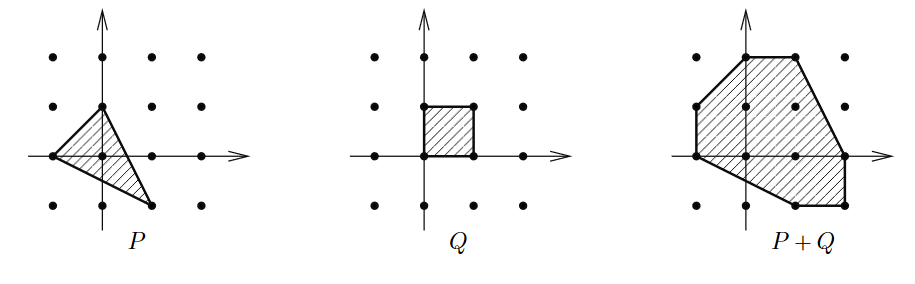
\includegraphics[scale = 0.7]{../images/image1.png}
        \caption{Examples of $P$, $Q$, and $P+Q$}
    \end{center}
\end{figure}

As an abuse of notation, when we add a subset $X \subset \RR^n$ to a singleton $\{v\} \subset \RR^n$ where $v \in \RR^n$, we will sometimes denote their sum by $X + v$ without the curly braces. Geometrically, we are translating the subset $X$ by the vector $v$. The next definition will be about affine spaces. In Problem~\ref{problem-affine}, you will prove that affine spaces are simply translated vector subspaces. 

\begin{defn}
    We call a space $A \subset \RR^n$ an \textbf{affine space} if the line through any pair of points $x, y \in A$ is contained in $A$. That is, for all $x, y \in A$ and $\lambda \in \RR$, we have $\lambda x + (1 - \lambda)y \in A$. 
\end{defn}

\begin{prob}[10 points]\label{problem-affine}
    If $A \subset \RR^n$ is an affine space, prove that there exists a (non-necessarily unique) vector $v \in \RR^n$ and a unique vector subspace $V \subset \RR^n$ such that $A = v + V$. 
\end{prob}

Similar to vector subspaces, for every subset $S \subset \RR^n$ there exists a ``smallest" affine space which contains $S$. You may take this result for granted. 

\begin{defn} \label{definition-affine-span}
    For a non-empty subset of vectors $S \subset \RR^n$, there exists an affine space $\aff S$ containing $S$ such that if $W_0$ is an affine space containing $S$, then $\aff S \subset W_0$. We call $\aff S$ the \textbf{affine span} or \textbf{affine hull} of $S$. 
\end{defn}

\begin{remark}
    To be consistent with our naming, we call a linear combination of the form $\lambda_1 x_1 + \ldots + \lambda_m x_m$ where $\lambda_1 + \ldots + \lambda_m = 1$ an \textbf{affine combination} of the vectors $x_1, \ldots, x_m$. Then, it is not hard to show that $\aff S$ contains all affine combinations of elements in $S$. 
\end{remark}

Since $\RR$ is an infinite set, all non-trivial vector spaces will consist of an infinite number of vectors. Hence, we cannot compare the relative sizes of vector vectors based on the number of vectors in the space. However, when we consider the vector subspaces of for example $\RR^3$, we find subspaces that look like lines and planes through the origin. Intuitively, there should be a notion of dimension that allows us to say that the line will be ``smaller" than the plane. Now, we will develop our definition of the dimension of a vector space. 

\begin{defn}
    The vectors $v_1, \ldots, v_m \in V$ are said to be \textbf{linearly independent} if the only choice of constants $\lambda_1, \ldots, \lambda_m \in \RR$ satisfying $\sum_{i = 1}^m \lambda_i v_i = 0$ is $\lambda_1 = \ldots = \lambda_m = 0$. 
\end{defn}

Conversely, if there exist constants $\lambda_1, \ldots, \lambda_m \in \RR$ not all zero with $\sum_{i = 1}^m \lambda_i v_i = 0$, then we say that the vectors $v_1, \ldots, v_m$ are \textbf{linearly dependent}. 

\begin{prob}[5 points] \label{problem-linear-independence-uniqueness}
    Suppose that the vectors $v_1, \ldots, v_m \in V$ are linearly independent. Prove that every vector in $\lin \{v_1, \ldots, v_m\}$ can be written uniquely as a linear combination of $v_1, \ldots, v_m$. 
\end{prob}

One interpretation of the dimension of a vector space is the number of vectors needed to specify all the data in the space. For example, one vector is needed to specify a line and two vectors are needed to specify a plane. The uniqueness of representation in terms of linearly independent vectors given in Problem~\ref{problem-linear-independence-uniqueness} then motivates a definition of dimension in terms of the size of a set of linearly independent vectors. 

\begin{defn} \label{definition-basis}
    A set of linearly independent vectors is \textbf{maximal} if there is no larger set of linearly independent vectors which contain this set. Any such maximal set is called a \textbf{basis} of the vector space. 
\end{defn}

We would like to define the dimension of a vector space as the size of a basis. However, in order for this definition to be well-defined, we need that the number of elements in each basis is the same, which is not immediately obvious. Luckily this is the case. You may black-box the following result. 

\begin{thm}
    Let $V$ be a vector space. If there exists a basis with a finite number of elements, then all bases of $V$ have the same number of elements. 
\end{thm}

This allows us to define the dimension of not only vector spaces, but also affine spaces. 

\begin{defn} [Dimension of Vector Spaces and Affine Spaces]
    Let $V$ be a vector space. We define $\dim V$ to be the number of elements in a basis of $V$ whenever the basis is finite and $\infty$ otherwise. Let $A$ be an affine space. From Problem~\ref{problem-affine}, there exists a unique vector space $V$ that is a translate of $A$. We define $\dim A := \dim V$. We call $\dim V$ and $\dim A$ to be the \textbf{dimension} of $V$ and $A$, respectively. 
\end{defn}

\begin{prob} [5 points]
    Prove that $\dim \RR^n = n$. 
\end{prob}

\begin{example}
    In $\RR^3$, the subspaces of dimension $2$ are the planes passing through the origin and the subspaces of dimension $1$ are the lines passing through the origin. The only subspace of dimension $3$ is $\RR^3$. These are all the non-trivial subspaces of $\RR^3$.
\end{example}
\begin{figure}[h]
\begin{center}
    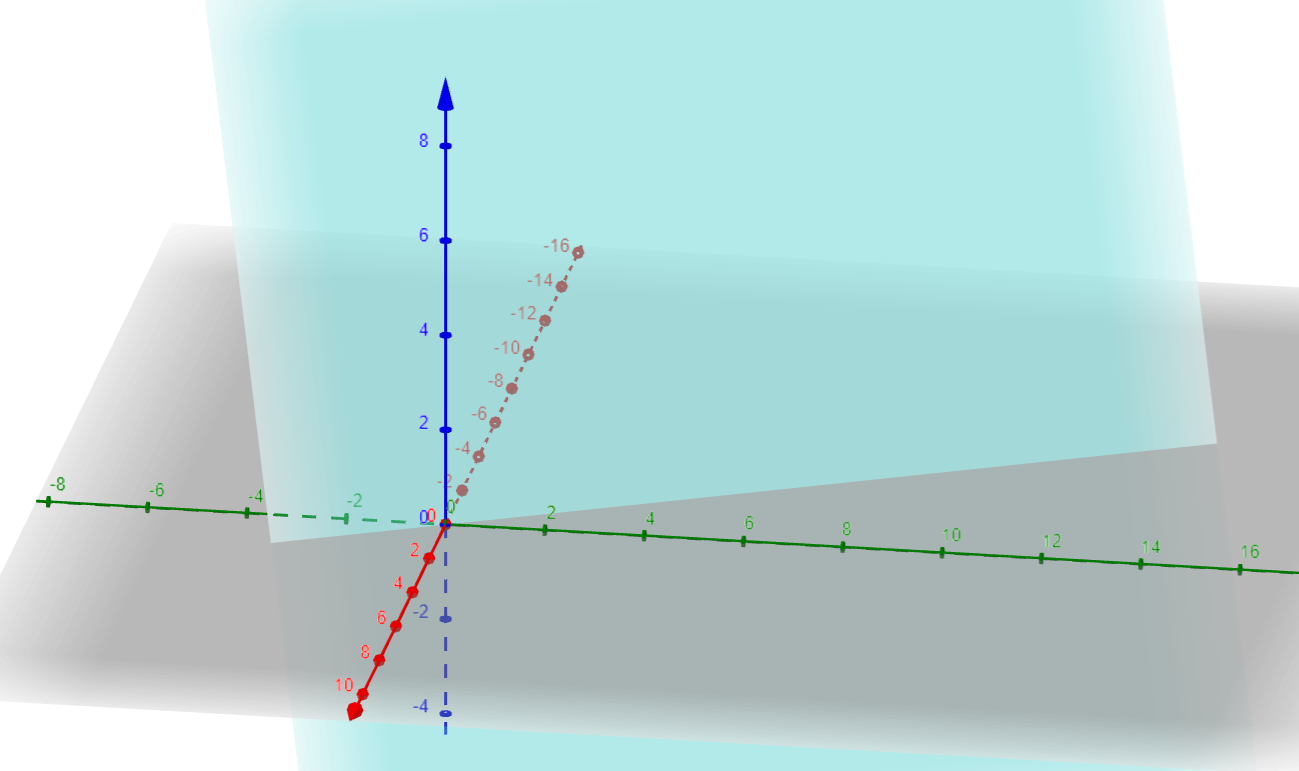
\includegraphics[scale = 0.3]{../images/image2.png}
    \caption{Example of a two-dimensional subspace (plane) of $\RR^3$}
\end{center}
\end{figure}

\begin{defn}
    Let $e_1, \ldots, e_n \in \RR^n$ be the vectors where $e_i$ is $1$ in the $i$th coordinate and $0$ everywhere else. Then $e_1, \ldots, e_n$ is a basis called the \textbf{standard basis} of $\RR^n$. 
\end{defn}

\subsection{Geometry}

We now explore the geometry of $\RR^n$ through the lens of an inner product. The inner product will allow us to compute lengths, angles, and projections. We first give the abstract definition of an inner product. 

% taken from Axler
\begin{defn} \label{definition-inner-product}
    An \textbf{inner product} on $V$ is a function that takes each ordered pair $(u, v)$ of elements in $V$ to a number $\langle u, v \rangle \in \RR$ with the following properties:
    \begin{enumerate}[label = (\roman*)]
        \item (Positive-Definiteness) $\langle v, v \rangle \geq 0$ for all $v \in V$ and $\langle v, v \rangle = 0$ if and only if $v = 0$. 
        \item (Linearity in the First Variable) $\langle \lambda u + v, w \rangle = \lambda \langle u, w \rangle + \langle v, w \rangle$ for all $u, v, w \in V$. 
        \item (Symmetry) $\langle u, v \rangle = \langle v, u \rangle$ for all $u, v \in V$.
    \end{enumerate}    
\end{defn}
\begin{prob} [10 points] \label{problem-standard-inner-product}
    On the vector space $\RR^n$, prove that the function $\langle \cdot, \cdot \rangle_2 : \RR^n \times \RR^n \to \RR$ defined as 
    \[
        \langle x, y \rangle_2 := \sum_{i = 1}^n x_i y_i. 
    \]
    is an inner product. 
\end{prob}
From now on, when we write an inner product $\langle \cdot, \cdot \rangle$ on $\RR^n$ without specifying the inner product, we will default to the standard inner product $\langle \cdot, \cdot \rangle_2$. With respect to this inner product, we can also define the \textbf{Euclidean norm}
\[  
    \norm{x} := \norm{x}_2 = \sqrt{\langle x, x \rangle} = \sqrt{\sum_{i = 1}^n x_i^2}.
\]
Geometrically, $\langle x, y \rangle$ is the (scaled) length of the projection of $y$ onto $x$ and $\norm{x}$ is the length of the vector $x$. Hence, the geometric meaning of $\langle x, y \rangle = 0$ is that the vectors $x$ and $y$ are orthogonal. In many situations, we want to work with a basis in which any two basis vectors are orthogonal and every basis vector has unit length.
\begin{defn}
    We say $v_1, \ldots, v_n \in V$ is an \textbf{orthonormal basis} of the vector space $V$ with respect to an inner product $\langle \cdot, \cdot \rangle$ if it is a basis, $\langle v_i, v_j \rangle = 0$ for $i \neq j$, and $\langle v_i, v_i \rangle = 1$. 
\end{defn} 

An orthonormal basis allows us to represent every vector as a linear combination of the basis vectors in terms of the inner product. 

\begin{prob} [5 points]
    Let $V$ be a vector space and $u_1, \ldots, u_n$ be an orthonormal basis with respect to an inner product $\langle \cdot, \cdot \rangle$. Then, for every $v \in V$, prove that 
    \[
        v = \sum_{k = 1}^n \langle v, u_k \rangle u_k. 
    \]  
\end{prob}

\begin{example}[The Gram-Schmidt Process]
    An inner product gives us an easy way to construct an orthonormal basis starting from any basis. Indeed, begin with a nonzero $v_1 \in V$. Suppose we have constructed linearly independent vectors $v_1, ..., v_m$ which are mutually orthogonal. If $\lin \{v_1, ..., v_m\}$ is the whole vector space, then this set is already a basis. Otherwise, there exists some vector $w \in V$ which is not in the linear span. Consider the vector 
    \[
        v_{m+1} = w - \sum_{k = 1}^m \langle w, v_k \rangle v_k.
    \]  
    You can check that this is non-zero and orthogonal to the previous vectors. Continue this process until our vectors span the whole vector spaces. After normalizing our vectors, we have an orthonormal basis. This process is called the \textbf{Gram-Schmidt process}. Thus, when working with a vector space with an inner product, we can always pick an orthonormal basis. 
\end{example}

\begin{prob} [10 points]
    Consider the inner product on $\RR^3$ defined by
    \[
        \langle x, y \rangle := x_1 y_1 + 2 x_2y_2 + 3 x_3y_3.
    \]
    Find an orthonormal basis of $\RR^3$ with respect to this inner product.
\end{prob}

\subsection{Linear Transformations}

Now that we have developed vector spaces, we should also be interested in the structure-preserving maps (morphisms) between them. These maps are called linear transformations or linear maps. 

\begin{defn}
    For two vector spaces $V, W$ we call $T : V \to W$ a \textbf{linear map} if $T(\lambda v+ \mu w) = \lambda T(v) + \mu T(w)$ for all $\lambda, \mu \in \RR$ and $v, w \in V$. 
\end{defn}

\begin{example}[Constructing Linear Maps] \label{example-linear-map-construction}
    Once you have a basis, linear maps are easy to construct. Suppose we were trying to create a linear map $T : V \to W$. Let $v_1, \ldots, v_n$ be a basis of $V$. Then, for any arbitrary vectors $w_1, \ldots, w_n$, there exists a unique linear map $T : V \to W$ satisfying $T(v_i) = w_i$ for all $1 \leq i \leq n$. Hence, the image of the basis vectors are sufficient to describe the whole map. 
\end{example}


Suppose we have a map $T : V \to W$ and fix bases $v_1, \ldots, v_n \in V$ and $w_1, \ldots, w_m \in W$. Then there are constants $a_{ji} \in \RR$ such that 
\[
    T(v_i) = \sum_{j = 1}^m a_{ji} \cdot w_j.
\]
From Example~\ref{example-linear-map-construction}, the entire data of $T$ is described by the images the $v_i$. Hence, the constants $a_{ji}$ are sufficient to describe the map $T$ completely. A compact way to store this data is in a $m \times n$ matrix: 
\[
    [a_{ij}] = \begin{pmatrix}
        a_{11} & a_{12} & \ldots & a_{1n} \\
        a_{21} & a_{22} & \ldots & a_{2n} \\
        \vdots & \vdots & \ddots & \vdots \\
        a_{m1} & a_{m2} & \hdots & a_{mn}
    \end{pmatrix}.
\]
Visually, a matrix is simply a rectangular table of numbers. However, it hides two additional pieces of data: a basis of $V$ and a basis of $W$. A matrix represents a linear map from $V$ to $W$ with respect to this chosen basis for $V$ and for $W$. Hence, the construction in Example~\ref{example-linear-map-construction} represents the linear map $T$ with respect to the basis $\{v_i\}_{1 \leq i \leq n}$ and the basis $\{w_i\}_{1 \leq i \leq m}$. For a fixed map $T : V \to W$, the corresponding matrix will change based on which basis we choose for $V$ and $W$. 
\begin{remark} 
    In the correspondence between matrices and linear maps, whenever we write down a $m \times n$ matrix, we will implicitly assume that it is representing a map $T : \RR^n \to \RR^m$ with respect to the standard bases. 
\end{remark}
\begin{example}
    The matrix $\begin{pmatrix} 1 & 2 \\ 3 & 4 \end{pmatrix}$ represents the map $T : \RR^2 \to \RR^2$ defined by $T(e_1) = e_1 + 3e_2$ and $T(e_2) = 2e_1 + 4e_2$. 
\end{example}

Given a map $T : V \to W$, there are two associated vector subspaces. 
\begin{defn}
    Let $T : V \to W$ be a linear map. Define the subspaces 
    \begin{align*}
        \ker T & := T^{-1}(0) = \{v \in V : T(v) = 0\} \\
        \im T & := T(V) = \{w \in W : \exists v \in V \text{ such that } T(v) = w\}.
    \end{align*}
    We call $\ker T$ the \textbf{kernel} of $T$ and $\im T$ the \textbf{image} of $T$. 
\end{defn}

The kernel and image satisfy the following theorem, which you may take as a black box. 
\begin{thm}
    Let $T : V \to W$ be a linear map where $V$ is finite-dimensional. Then $\dim V = \dim \ker T + \dim \im T$. 
\end{thm}

\begin{prob} [10 points]
    Let $v_1, ..., v_n \in \RR^n$ be a basis and let $\alpha_1, ..., \alpha_n \in \RR$ be real numbers. Prove that there is exactly one vector $w \in \RR^n$ that satisfies 
    \[
        \langle v_i, w \rangle = \alpha_i    
    \]
    for all $1 \leq i \leq n$. 
\end{prob}
\subsection{Spectral Theory}
\begin{defn}
    Let $T : V \to V$ be a linear map. Suppose there exists a non-zero $v$ and constant $\lambda \in \RR$ such that $Tv = \lambda v$. Then we call $\lambda$ an \textbf{eigenvalue} and $v$ an \textbf{eigenvector} with eigenvalue $\lambda$. 
\end{defn}

As an example, consider the linear map $T : \RR^2 \to \RR^2$ defined by $T(e_1) = e_1 + 2e_2$ and $T(e_2) = 2e_1 + e_2$. This has eigenvector $e_1 + e_2$ because $T(e_1 + e_2) = 3 (e_1 + e_2)$. The corresponding eigenvalue is $3$. Note that linear maps do not necessarily have (real) eigenvalues / eigenvectors. For example, consider the map $T : \RR^2 \to \RR^2$ defined by $T(e_1) = e_2$ and $T(e_2) = -e_1$. Geometrically, it is easy to see why this map has no real eigenvectors since it is a rotation. 

\begin{defn}
    We call a linear map $T : V \to V$ \textbf{self-adjoint} with respect to an inner product $\langle \cdot, \cdot \rangle$ if for all $x, y \in V$ we have 
    \[
        \langle x, Ty \rangle = \langle Tx, y \rangle.     
    \]
\end{defn}

One easy example of a subset of the self-adjoint operators with respect to the standard inner product are the diagonal matrices, which are maps of the form $T(e_i) = \lambda_i e_i$ for $\lambda_i \in \RR$. Self-adjoint operators are nice because they are guarenteed to have many eigenvectors. Indeed, you may take the following result as a black box. 

\begin{thm}
    Suppose $T : \RR^n \to \RR^n$ is self-adjoint with respect to some inner product on $\RR^n$. Then there exists an orthonormal basis of eigenvectors with real eigenvalues. 
\end{thm}

Let $A : \RR^n \to \RR^n$ be a linear map with inner product $\langle \cdot, \cdot \rangle$. We say $A$ is \textbf{positive semi-definite} if $A$ is self-adjoint with respect to the inner product and $\langle x, Ax \rangle \geq 0$ for all $x \in \RR^n$. In the following problem, you will prove some properties of self-adjoint linear maps. 

\begin{prob}[25 points]
    Let $A : \RR^n \to \RR^n$ be a self-adjoint linear map with respect to some inner product $\langle \cdot, \cdot \rangle$. 
    \begin{enumerate}[label = (\alph*)]
        \item (15 points) Let $\lambda$ be the largest eigenvalue of $A$. Prove that 
        \[
            \lambda = \sup_{x \neq 0} \frac{\langle x, Ax \rangle}{\langle x, x \rangle}.
        \]
        For a definition of $\sup$, look at Definition~\ref{defn-supremum}.

        \item (10 points) If $A$ is positive semi-definite, prove that 
        \[
            \langle x, Ay \rangle^2 \leq \langle x, Ax \rangle \cdot \langle y, Ay \rangle 
        \]
        for all $x, y \in \RR^n$.
    \end{enumerate}
    
\end{prob}

When you drop the positive semi-definiteness condition, the inequality does not necessarily hold, and can even reverse!

\begin{prob} [50 points]
    Suppose that $A : \RR^n \to \RR^n$ is self-adjoint with respect to some inner product $\langle \cdot, \cdot \rangle$. Prove that the following two conditions are equivalent:
    \begin{enumerate}[label = (\roman*)]
        \item The space spanned by the eigenvectors with positive eigenvalues has dimension at most $1$.
        \item Whenever $\langle y, Ay \rangle \geq 0$, we have $\langle x, Ay \rangle^2 \geq \langle x, Ax \rangle \langle y, Ay \rangle$ for all $x$. 
    \end{enumerate}
\end{prob}

The eigenvalues of matrices obtained from graphs also satisfy nice properties. We call a matrix $M$ a \textbf{graphic matrix} if there is a connected graph $G$ with vertices $\{1, \ldots, n\}$ such that $M = [M_{ij}]$ where $M_{ij} = 0$ whenever $\{i, j\} \notin E(G)$ and $M_{ij} > 0$ otherwise. We summarize the needed results of these matrices in Theorem~\ref{theorem-graphic-matrices}. In this theorem, we introduce the notion of the transpose of a matrix. If $M$ is a $n \times n$ matrix $[M_{ij}]_{1 \leq i, j \leq n}$, we define the \textbf{transpose} of $M$ to be $M^T = [M_{ji}]_{1 \leq i, j \leq n}$. Visually, $M^T$ is $M$ with the entries reflected across the main diagonal. In the vector space world, $M^T$ has a natural interpretation as the matrix of the dual of the represented linear map, but this knowledge is not required for the power round. 

\begin{thm} \label{theorem-graphic-matrices}
    Let $M : \RR^n \to \RR^n$ be a graphic matrix. Then, the following results are true. 
    \begin{enumerate}[label = (\alph*)]
        \item $M$ has a positive eigenvalue $\lambda > 0$ that is greater than any other (real) eigenvalue. 
        \item The subspace of eigenvectors of eigenvalue $\lambda$ is one-dimensional and contains the unique eigenvector (up to scalar factor) with strictly positive entries. 
        \item $M^T$ also has an eigenvector with strictly positive entries with respect to the eigenvalue $\lambda$. 
    \end{enumerate}
\end{thm}

The next problem is an application of Theorem~\ref{theorem-graphic-matrices}. In the language of Markov chains, it states that every nice Markov chain has a unique stationary distribution. 

\begin{prob} [15 points]
    Suppose that there are $n$ lily pads numbered $1, \ldots, n$ on a pond and numbers $0 < p_{ij} < 1$ for $1 \leq i, j \leq n$ such that $\sum_j p_{ij} = 1$ for all $1 \leq i \leq n$. Aleksa, being an enjoyer of aquatic plants, asks you to come up with an $n$-tuple $(\pi_1, \ldots, \pi_n)$ where $\pi_1, \ldots, \pi_n \geq 0$ and $\pi_1 + \ldots + \pi_n = 1$. With probability $\pi_i$, Aleksa will initially step onto lily pad $i$. From then on, if Aleksa is on lily pad $j$ for some $1 \leq j \leq n$, he will move to lily pad $k$ with probability $p_{jk}$ and rest there for a second. Prove that there exists a unique $n$-tuple $(\pi_1, \ldots, \pi_n)$ that you can give to Aleksa such that at any time, the probability that he will be at lily pad $k$ is $\pi_k$ for all $1 \leq k \leq n$.
\end{prob}

\subsection{Determinants}

Now, suppose we want to know how a linear map $T : \RR^n \to \RR^n$ would change the volume of a object in $\RR^n$. To answer this question, we first consider a multi-linear map $D : (\RR^n)^n \to \RR$ satisfying the following three properties:
\begin{enumerate}[label = (\roman*)]
    \item (Multilinearity) For any $1 \leq i \leq n$, $v_i, v_i' \in \RR^n$ and $\lambda \in \RR$, we have 
    \begin{align*}
        D(\ldots, v_{i-1}, \lambda v_i + v_i', v_{i+1}, \ldots) = \lambda D(\ldots, v_{i-1}, v_i, v_{i+1}, \ldots ) + D(\ldots, v_{i-1}, v_i', v_{i+1}, \ldots).
    \end{align*}
    \item (Antisymmetry) For $1 \leq i < j \leq n$, let $\mathsf{swap}_{ij} : (\RR^n)^n \to (\RR^n)^n$ be the map that swaps the $i$ and $j$ vectors. Then $D(\mathsf{swap}_{ij}(v_1, \ldots, v_n)) = -D(v_1, \ldots, v_n)$ for all $1 \leq i < j \leq n$. 
    \item (Normality) $D(e_1, \ldots, e_n) = 1$ where $e_1, \ldots, e_n$ is the standard basis for $\RR^n$.
\end{enumerate}

Intuitively, $D$ is the (signed) volume for the parallelotope spanned by the vectors in its argument. In particular, condition (iii) says that the volume of a unit cube (oriented in the correct way) is $1$. You may use the following result without proof. 
\begin{thm}
    There exists a unique multilinear, antisymmetric, normal functional $D : (\RR^n)^n \to \RR$. 
\end{thm}

Using this functional $D$, we can define the determinant of a linear operator $T : \RR^n \to \RR^n$ as follows. 
\begin{defn}
    Let $T : \RR^n \to \RR^n$ be a linear map. We define the \textbf{determinant} of $T$ to be 
    \[
        \det T := D(Te_1, \ldots, Te_n)    
    \]
    where $e_1, \ldots, e_n$ is the standard basis of $\RR^n$. 
\end{defn}

The determinant enjoys many nice properties. Below, we have listed some of these properties which you may assume without proof.

\begin{prop}
    The determinant satisfies the following properties.   
\begin{enumerate}[label = (\roman*)]
    \item If $S, T : \RR^n \to \RR^n$ are two linear operators, then $\det (S \circ T) = (\det S) (\det T)$. 
    \item If $\lambda \in \RR$ and $T : \RR^n \to \RR^n$, then $\det (\lambda T) = \lambda^n \det (T)$. 
    \item $\det (I) = 1$ where $I : \RR^n \to \RR^n$ is the identity map. 
\end{enumerate}
\end{prop}

Closely related to the determinant is the \textbf{group of permutations} $S_n$ that consist of all bijective maps $\pi : [n] \to [n]$. In the following problem, you will consider special maps $\chi : S_n \to \{-1, 1\}$. 

\begin{prob} [30 points]
    We call a map $\chi : S_n \to \{-1, 1\}$ a \textbf{character} (of $S_n$) if $\chi(\pi_1 \circ \pi_2) = \chi(\pi_1) \cdot \chi(\pi_2)$ for all $\pi_1, \pi_2 \in S_n$. Prove that there are exactly two characters of $S_n$ when $n \geq 2$.  
\end{prob}

From the previous problem, we know that $S_n$, when $n \geq 2$, has two characters which we denote by $\1_{S_n}$ and $\sgn$. The former is simply the map which sends every permutation to $1$ and the latter is the \textbf{sign representation} of $S_n$ which sends transpositions (permutations which simply swap two elements) to $-1$. When $n = 1$, it is easy to see that there is only one character $\1_{S_n}$. In that case, we will let $\sgn = \1_{S_n}$. The $\sgn$ character gives us the following explicit formula for the determinant of a linear map. 

\begin{prop}
    If $[a_{ij}]$ is the matrix for a linear map $T : \RR^n \to \RR^n$, then 
    \[
        \det T := \sum_{\pi \in S_n} \sgn(\pi) \prod_{i = 1}^n a_{i \pi(i)}.
    \]
\end{prop}
    
In the right hand side, we are picking $n$ terms entries in the matrix which are all in distinct rows and columns and multiplying them together. Then we are adding all of these products while weighting them based on the sign of our permutation. 

\begin{prob}[Computing Determinants, 30 points]
    In this exercise, you will compute a few determinants. 
    \begin{enumerate}[label = (\alph*)]
        \item (5 points) Compute the determinant of $\begin{bmatrix} 1 & 2 & 3 \\ 4 & 5 & 6 \\ 7 & 8 & 9 \end{bmatrix}$. 
        \item (10 points) Let $v_1, \ldots, v_n$ be a collection of linearly dependent vectors. Compute $D(v_1, \ldots, v_n)$. 
        \item (15 points) Let $v_1, \ldots, v_n$ be an orthonormal basis of $\RR^n$. Compute $|D(v_1, \ldots, v_n)|$. 
    \end{enumerate}
\end{prob}

In Problem~\ref{computing-volumes}(c), you will prove that the determinant is indeed the volume of the parallelotope spanned by the $n$ column vectors. For the final concept in this subsection, we define a minor of a matrix. 

\begin{defn}
    Let $M$ be a matrix, not necessarily square. We define a \textbf{minor} of the matrix $M$ to be the determinant of some smaller square matrix which we obtain by deleting rows and columns. 
\end{defn}

To give an example, consider the matrix 
\[
    A = \begin{pmatrix}
         1 & 2 & 3 \\
         4 & 5 & 6 \\
    \end{pmatrix}.   
\]
The minors of $A$ will be the determinants of the following matrices
\[
    \begin{pmatrix}
        1 & 2 \\ 4 & 5
    \end{pmatrix}, \begin{pmatrix} 1 & 3 \\ 4 & 6 \end{pmatrix}, \begin{pmatrix} 2 & 3 \\ 5 & 6 \end{pmatrix}
\]
and each individual entry in $A$. 

\begin{defn} \label{unimodular}
    Let $M$ be a matrix. We say $M$ is \textbf{unimodular} if all of its minors are in $\{-1, 0, 1\}$. 
\end{defn}

The next time Definition~\ref{unimodular} will reppear is at Section~\ref{subsection-matroids}. Thus, you do not need to concern yourself with the definition at the moment. 

\subsection{Metric Spaces}
    In this section, we introduce the notion of a topology. A topology is gives us a way to characterize sets of points which are close together. We will only be interested in topologies which can be induced by a metric. With a metric, we can begin talking about continuity and convergence. 
    \begin{defn} \label{definition-metric-space}
        A \textbf{metric space} is an ordered pair $(X, d)$ of a set $X$ and a \textbf{metric} $d : X \times X \to \RR$ which satisfies 
        \begin{enumerate}[label = (\roman*)]
            \item $d(x, y) \geq 0$ for all $x, y \in X$ and $d(x, y) = 0$ if and only if $x = y$. 
            \item $d(x, y) = d(y, x)$ for all $x, y, \in X$. 
            \item $d(x, y) + d(y, z) \geq d(x, z)$ for all $x, y, z \in X$. 
        \end{enumerate}
    \end{defn}
    From the definition, we can see that a metric space includes two components: a set of points $X$ and a function $d$ called the metric. The metric $d$ should be thought of a measurement of distance between points. Definition~\ref{definition-metric-space}(iii) then asserts that the triangle inequality holds.
    \begin{example}
        On any set $X$, we can equip it with the discrete metric $\1 : X \times X \to \{0, 1\}$ defined by $\1(x, y) = 1$ if $x \neq y$ and $\1(x, y) = 0$ otherwise. 
    \end{example} 
    \begin{example}
        The pair $(\RR^n, d_2)$ where $d_2(x, y) = \norm{x-y}$ is the Euclidean norm is a metric space. More generally, $(\RR^n, d_p)$ where 
        \[
            d_p(x, y) = \left \{ \sum_{k = 1}^n |x_i - y_i|^p \right \}^{1/p}
        \] 
        and $p \geq 1$ is a metric space. When $p = 1$ and $n = 1$, we get the common metric space $(\RR, |\cdot|)$. This formalizes the notion of the absolute value being a measure of distance in the real numbers.  
    \end{example}

    \subsection{A Brief Detour: Supremum and Infimum}
    Before introducing more topological notions, we first introduce a property of many ordered sets which generalizes the idea of a maximum and minimum. This concept will be used regularly in later sections of the power round. 
    % definition from Rudin
    \begin{defn}\label{defn-supremum}
        Suppose $E \subset \RR$ is bounded above. If a real number $\alpha \in \RR$ satisfies the properties that 
        \begin{enumerate}[label = (\roman*)]
            \item $\alpha$ is an upper bound of $E$
            \item if $\alpha_0$ is an upper bound of $E$, then $\alpha_0 \geq \alpha$
        \end{enumerate}
        then, we call $\alpha$ a \textbf{supremum} of $A$. Similarly, we call $\beta$ an \textbf{infimum} of $E$ if $E$ is bounded below and $-\beta$ is a supremum of $-E$. Let $\sup E$ denote the set of suprema and $\inf E$ denote the set of infima. 
    \end{defn}

    \begin{prob} [5 points]
        Prove that for any subset $E \subset \RR$, if suprema or infima exist they must be unique. 
    \end{prob}

    It turns out that any subset of real numbers with an upper bound also has a well-defined supremum and any subset of real numbers with a lower bound also has a well-defined infimum. You may take this fact for granted. This allows us to make the following definition. 

    \begin{defn}
        Let $A \subset \RR$ be a subset of the reals. We define the $\sup A$ to be the supremum of $A$ if $A$ is bounded above and $\inf A$ to be the infimum of $A$ if $A$ is bounded below. If $A$ is not bounded above we let $\sup A = +\infty$. Similarly, if $A$ is not bounded below, we let $\inf A = -\infty$.   
    \end{defn}

    The supremum and infimum are generalizations of maximum and minimum to infinite sets. For example, the open interval $(1, 2)$ contains no element which is larger than all of the other elements or smaller than all of the other elements. This implies that the maximum and minimum are undefined for this set. However, we would like to say that the ``minimum" is $1$ and the ``maximum" is $2$. The supremum and infimum allow us to express this idea with $\sup (1, 2) = 2$ and $\inf (1, 2) = 1$. For another example, consider the set of increasingly precise decimal approximations of $\sqrt{2}$: $\{1, 1.4, 1.41, 1.414, 1.4142, ... \}$. This set has no maximum but it has supremum $\sqrt{2}$. In the following problem, you will prove an important analytic property of the supremum and infimum. We only state the result for supremum, but the corresponding result for infimum can be easily deduced. 

    \begin{prob} [5 points]
        Let $A \subset \RR$ be a subset with $\alpha = \sup A < \infty$. Prove that for every $\varepsilon > 0$, there exists an element $\beta \in A$ such that $\beta > \alpha - \varepsilon$. 
    \end{prob}

    However, in most applications, the supremum fulfills a similar role to the maximum. The following problem uses both, but the you may find that there is little difference between the supremum and the maximum in this example.  
    \begin{prob} [15 points]
        In probability theory, there is a useful metric on the distributions of a fixed sample space called the \textbf{total variation distance}. In this problem, we explore a simple case of this distance. Consider the simplex
        \[
            \Delta_d := \{(x_1, ..., x_d) \in \RR^d : x_1 + ... + x_d = 1 \text{ and } x_1, ..., x_d \geq 0\}.
        \]
        We define the total variation distance between two vectors $x, y \in \Delta_d$ to be 
        \[
            d_{\mathsf{TV}} (x, y) = \frac{1}{2}  \sum_{k = 1}^d |x_k - y_k|.
        \]
        \begin{enumerate}[label = (\alph*)]
            \item (5 points) Prove that $d_{\mathsf{TV}}$ is a metric.
            
            \item (10 points) Prove that 
            \[
                d_{\mathsf{TV}}(x, y) = \max_{A \subset [d]} \left | \sum_{n \in A} (x_n - y_n) \right | = \frac{1}{2}\sup \left \{ \sum_{k = 1}^d f_k (x_k - y_k) : \max_{i \in [d]} |f_i| \leq 1 \right \}
            \] 
        \end{enumerate}
    \end{prob}
    Now back to the regularly scheduled programming. 

    \subsection{Topology of Metric Spaces} 
    
    \begin{defn}
        Let $(X, d)$ be a metric space. For $r > 0$, we can define the following subsets of $X$:
        \begin{align*}
            B_0(x, r) & = \{y \in X : d(x, y) < r\} \\
            B(x, r) & = \{y \in X : d(x, y) \leq r \} \\
            S(x, r) & = \{y \in X : d(x, y) = r\}.
        \end{align*}  
        When the underlying metric space is understood to be $(\RR^n, \norm{\cdot})$, we let $B^n := B(0, 1)$ and $S^{n-1} := S(0, 1)$. 
    \end{defn}
    
    Geometrically, $B_0(x, r)$ is the open ball of radius $r$ and $S(x, r)$ is the sphere of radius $r$. The difference between $B(x, r)$ and $B_0(x, r)$ is that the former includes points which are exactly a distance of $r$ away while the latter does not. If we consider $\RR^2$ equipped with the standard Euclidean metric, the open ball centered around $0$ with radius $1$ would be a unit disk without boundary. However, if we change the metric, to say for example the taxicab metric, open balls would be a different shape. 

    \begin{prob} [5 points]
        On $\RR^2$, define the \textbf{taxicab distance} as $d_T(x, y) = |x_1 - y_1| + |x_2 - y_2|$. Describe or draw the shape of open balls of the taxicab distance. A picture suffices for this problem. 
    \end{prob} 

    In a metric space, the open balls generate a topology. It is not necessary for the power round for you to understand what this means, but morally it means that we have a means to understand continuity and convergence. In the following definitions, all terms apply to some metric space $(X, d)$. 

    \begin{defn}
        We call a subset $S \subset X$ an \textbf{open set} if and only if for each $s \in S$, there is a positive radius $r > 0$ such that $B_0(s, r) \subset S$. Trivially, the empty set and the whole set are always open. We call a subset $S \subset X$ a \textbf{closed set} if the complement $S^c$ is open.
    \end{defn}
    
    \begin{defn}
        Let $S \subset X$ be a subset of our metric space. 
        \begin{enumerate}[label = (\roman*)]
            \item The \textbf{interior} of $S$, denoted by $\tint (S)$, is the set of points $p \in S$ such that there exists an open ball containing $p$ and contained in $S$.

            \item The \textbf{boundary} of $S$, denoted by $\partial S$, is the set of points $p \in X$ such that any open ball centered around $p$ contains at least one point of $S \backslash \{p\}$ and at least one point in $S^c$. 

            \item The \textbf{closure} of $S$, denoted by $\clo (S)$, is defined as the union of $S$ and boundary of $S$. 
        \end{enumerate} 
    \end{defn} 
    \begin{remark}
        Suppose $(X, d)$ is a metric space. Then, any subset $S \subset X$ when equipped with the metric $d$ also becomes a metric space. Hence, for subsets $E \subset S$, we can consider the interior, boundary, and closure of $E$ \textit{relative} to $S$. This means that instead of viewing $E$ as a subset of the metric space $(X, d)$, we are viewing $E$ as a subset of the metric space $(S, d)$. This will give drastically different sets for the interior, boundary, and closure. Thus, we will denote by $\tint_S(E)$, $\partial_S E$, and $\clo_S(E)$ as the interior, boundary, and closure relative to $S$. 
    \end{remark}

    \begin{figure}[h]
        \begin{center}
            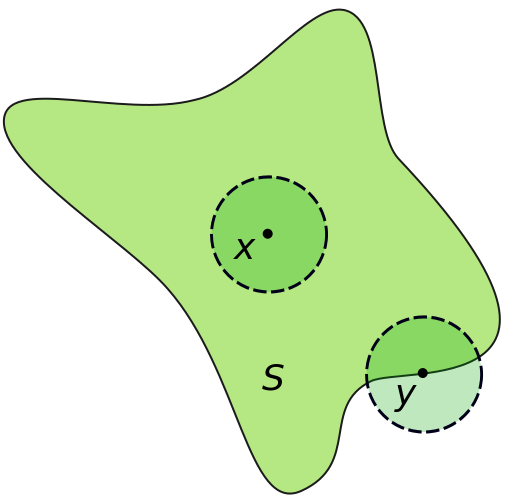
\includegraphics[scale = 0.2]{../images/image3.png}
            \caption{$x$ is an interior point while $y$ is a boundary point.}
        \end{center}
    \end{figure}

    \begin{prob} [10 points]
        Let $X = \RR^3$ and consider the subset $K = \{(x, y, z) \in \RR^3 : 0 \leq x, y \leq 1, z = 0 \}$. Let $P = \{(x, y, z) \in \RR^3 : z = 0\}.$ Please answer the following two questions. No proof of your answers are required. 
        \begin{enumerate}[label = (\alph*)]
            \item (5 points) What are $\tint K$, $\partial K$, and $\clo K$?
            \item (5 points) What are $\tint_P K$, $\partial_P K$, and $\clo_P K$?
        \end{enumerate}
    \end{prob}
    For nice shapes in Euclidean space, the interior, boundary, and closure are exactly what you would imagine them to be. For example, the interior of an open disk would be itself. The boundary would be the circle bounding the disk. The closure would be the closed disk. However, for more irregular shapes it might be wise to rely less on your intuition. The following is an alternative characterization of the closure and interior which you do not need to prove. 

    \begin{prop}[Alternative Characterization of Interior and Closure]
        Let $E \subset X$ be a subset. Prove that $\tint E$ is the largest open set contained in $E$ and $\clo E$ is the smallest closed set containing $E$. In other words, prove that $\tint E$ is open, $\clo E$ is closed, and whenever $\mcO \subset E$ is open and $\mcC \supset E$ is closed, then 
        \[
            \mcO \subset \tint E \subset E \subset \clo E \subset \mcC.
        \]
    \end{prop}

    One way to construct metric spaces is to build them up from smaller ones. In particular, if $(X, d_X)$ and $(Y, d_Y)$ are metric spaces, we can construct a metric space $(X \times Y, d)$ where the metric is defined by 
    \[
        d ( x_1 \times y_1, x_2 \times y_2) = \sqrt{d_X(x_1, x_2)^2 + d_Y(y_1, y_2)^2}.
    \] 
    We leave it as an exercise to prove that this is indeed a metric. Note that the metric space $(\RR^n, \norm{\cdot})$ is constructed exactly in this way. 

    \begin{defn} \label{definition-convergence-cauchy}
        We say a sequence of points $\{a_n\}_{n\geq 1} \subset X$ \textbf{converges} to a point $a \in X$ if for every $\varepsilon > 0$, there exists a positive constant $N$ such that for all $n > N$, we have $d(a_n, a) < \varepsilon$. We write this as $a_n \to a$ as $n \to \infty$ or $\lim_{n \to \infty} a_n = a$. We say the sequence $\{a_n\}_{n \geq 1}$ is \textbf{Cauchy} if for every $\varepsilon > 0$, there exists a positive constant $N$ such that for all $m, n > N$, we have $d(a_n, a_m) < \varepsilon$.  
    \end{defn}

    Definition~\ref{definition-convergence-cauchy} is a formalization of the idea a sequence of points getting ``close" to a limit. Not only do our points need to get arbitrarily close to the limit, but they have to eventually stay arbitrarily close as well. A Cauchy sequence is similar to a convergent sequence, except we are only guarenteed that our sequence gets (and eventually stays) arbitrarily close to itself. Convergent sequences are always Cauchy sequences, but the converse is not necessarily true. Indeed, see if you can find a sequence in the rationals $\QQ$ that is Cauchy but not convergent. However, in many spaces that we work with, the two notions are the same. The name of such spaces is given in Definition~\ref{definition-complete}.

    \begin{defn}\label{definition-complete}
        We call a metric space $(X, d)$ \textbf{complete} if all Cauchy sequences in $X$ converge. 
    \end{defn}
    \begin{prob} [30 points] The following two problems involve the convergence of sequences. 
        \begin{enumerate}[label = (\alph*)]
            \item (10 points) Prove that every convergent sequence has a unique point of convergence. That is, if $a_n \to x_1$ and $a_n \to x_2$ are two convergent sequences in a metric space $(X, d)$, then $x_1 = x_2$.
            \item (20 points) Let $(X, d)$ be a complete metric space. Let $f : X \to X$ be a map satisfying $d(f(x), f(y)) \leq c \cdot d(x, y)$ where $c \in (0, 1)$. Prove that there exists exactly one $x_{\mathsf{fix}} \in X$ with $f(x_{\mathsf{fix}}) = x_{\mathsf{fix}}$. 
        \end{enumerate}
    \end{prob}
     
    The next definition is a topological generalization of finiteness and will be particularly important for the remainder of the power round.

    \begin{defn}\label{definition-compactness}
        A subset $K \subset X$ is \textbf{compact} if for any collection of open sets $\{U_\alpha\}_{\alpha \in I}$ satisfying
        \[
            K \subset \bigcup_{\alpha \in I} U_\alpha
        \] 
        there exists a finite subset $S \subset I$ with 
        \[
            K \subset \bigcup_{\alpha \in S} U_\alpha.
        \]  
        Written succinctly, every open cover of $K$ has a finite subcover. 
    \end{defn}

    Whenever we are in $\RR^n$, the open covers in Definition~\ref{definition-compactness} can be avoided with the following characterization of compact sets. You may assume the result without proof. 

    \begin{thm} \label{theorem-heine-borel}
        A subset $K \subset \RR^n$ is compact if and only if $K$ is closed and bounded.  
    \end{thm}

    In a metric space $(X, d)$, we say that a subset $K \subset \RR^n$ is bounded if there exists $r \in \RR_{> 0}$ and $x \in X$ such that $K \subset B(x, r)$. In other words, there exists a ball of finite radius which covers the set. Another result about compact sets is that given any open cover, any small enough subset will be contained in a single open set in the open cover. We summarize this result in the following theorem. 

    \begin{thm}
        Let $\mathcal{A}$ be an open covering of the metric space $(X, d)$. If $X$ is compact, there is a $\delta > 0$ such that for every subset of $X$ having diameter less than $\delta$, there exists an element of $\mathcal{A}$ containing it. Recall that the diameter of the subset $E$ is defined as 
        \[
            \diam E := \sup_{x, y \in E} d(x, y). 
        \]
    \end{thm}
    We now consider the maps between metric spaces which preserve their topology. 
    
    \begin{defn} \label{definition-continuity}
        Given metric spaces $(X, d_X)$ and $(Y, d_Y)$, we call a map $f : X \to Y$ \textbf{continuous} if $f^{-1}(U)$ is open as a subset of $X$ whenever $U \subset Y$ is open as a subset of $Y$. A \textbf{continuous function} is then a map $f : X \to \RR$ where $\RR$ is equipped with the Euclidean metric. 
    \end{defn}
    
    When given an explicit formula for a map, Definition~\ref{definition-continuity} may be a bit cumbersome to use. Luckily, we have the following $\varepsilon$-$\delta$ definition of continuity which in some situations is more suited to computation. You may take this result for granted.

    \begin{prop}
        A map $f : (X, d_X) \to (Y, d_Y)$ between metric spaces is continuous if and only if for any $x \in X$ and $\varepsilon > 0$, there exists a $\delta := \delta(x, \varepsilon) > 0$ dependent on both $x$ and $\varepsilon$ such that for all $u \in X$, we have
        \[
            d_X(x, u) < \delta \implies d_Y(f(x), f(u)) < \varepsilon. 
        \]
        In other words, we can make the value $f(u)$ get arbitrarily close to $f(x)$ as long as $u$ is sufficiently close to $x$.
    \end{prop}

    \begin{prob}[Exercises in Continuity and Compactness, 40 points]
        Let $(X, d)$ be a metric space.
        \begin{enumerate}[label = (\alph*)]
            \item (10 points) Let $K \subset X$ be compact and $f : (X, d) \to (M, d_M)$ be a continuous map. Prove that $f(K)$ is a compact subset of $M$.
            \item (10 points) Suppose we have a sequence of non-empty compact subsets $K_n \subset X$ satisfying $K_n \supset K_{n+1}$ for all $n \geq 1$. Prove that $\bigcap_{n \geq 1} K_n$ is non-empty and compact. 
            \item (10 points) Let $\{x_n\} \subset \RR^n$ be a bounded sequence. Prove that there is a convergent subsequence.
            \item (10 points) Let $K \subset X$ be compact and $f : K \to \RR$ a continuous function. Prove that there exists $x_{\mathsf{min}}, x_{\mathsf{max}} \in K$ that satisfy
            \begin{align*}
                    f(x_{\mathsf{min}}) = \inf_{x \in K} f(x), \quad f(x_{\mathsf{max}}) = \sup_{x \in K} f(x). 
            \end{align*}
        \end{enumerate}    
    \end{prob}
    
\newpage 

\section{Convex Bodies}
\subsection{Properties of Convex Sets}

\begin{defn}\label{definition-convex-set}
 A set $C \subset \RR^n$ is \textbf{convex} if for any two elements $x, y \in C$, the set $C$ contains the segment $[x, y]$. That is, for all $\alpha \in [0, 1]$, we have $\alpha x + (1-\alpha) y \in C$. 
\end{defn}

A familiar class of convex sets are the affine spaces. Since an affine space $A$ is defined to be a space for which for any two $x, y \in A$ and $\lambda \in \RR$ satisfies $\lambda x + (1-\lambda)y \in A$, it is clear that affine spaces are convex. Convex sets have a construction similar to that of Definition~\ref{definition-linear-span}.

\begin{defn} \label{definition-convex-hull}
    For a non-empty subset of vectors $S \subset \RR^n$, there exists a convex set $\conv S$ containing $S$ such that if $C_0$ is a convex set containing $S$ then $\conv S \subset C_0$. We call $\conv S$ the \textbf{convex hull} of $S$.
\end{defn}

\begin{remark}
By generalizing the linear combination in Definition~\ref{definition-convex-set}, we say a vector $x \in \RR^n$ is a \textbf{convex combination} of vectors $x_1, ..., x_m \in \RR^n$ if there are non-negative constants $\lambda_1, ..., \lambda_m \in \RR_{\geq 0}$ satisfying 
\[
    x = \sum_{i = 1}^m \lambda_i x_i \quad \text{ and } \quad \sum_{k = 1}^m \lambda_k = 1.
\]
It is not difficult to prove that $\conv S$ can be explicitly described as the set of points which can be represented as the convex combination of a finite set of points in $S$. From here on out, you may use this result as a black box. 
\end{remark}

We have finally come to the main objects that we will be working with in the power round. We will not be working with sets that are only convex. Instead, we will be working with sets that are convex \textit{and} compact. 

\begin{defn}
    A \textbf{convex body} is a non-empty convex and compact subset of $\RR^n$ for some $n \geq 1$. We let $\mathsf{K}^n$ denote the family of convex bodies in $\RR^n$. For $K \in \mathsf{K}^n$ we can define the \textbf{dimension} of $K$ as $\dim K := \dim \aff K$. 
\end{defn}

\begin{prob} [10 points] \label{problem-empty-interior}
    If $K \in \mathsf{K}^n$, prove that $\dim K < n$ if and only if $\tint K = \emptyset$. 
\end{prob}

Problem~\ref{problem-empty-interior} shows that there are a large class of non-trivial convex bodies in $\RR^n$ with empty interior. This makes topologically distinguishing convex objects tricky. For example, consider a closed square. In $\RR^2$ it has non-empty interior but in $\RR^3$ it has empty interior. Thus, to study the structure of convex bodies, we need the following refined notion of interior and boundary. 

\begin{defn} \label{definition-relint-relbd}
    Let $K \subset \RR^n$ be a convex body. Define
    \begin{align*}
        \rint K & = \tint_{\aff K} K \\
        \rbd K & = \partial_{\aff K} K
    \end{align*}
    where we take the interior and boundary while taking $\aff K$ to be the ambient space. 
\end{defn}

\begin{prob} [15 points]
    Let $K \subset \RR^n$ be a convex body. Let $x \in \rint K$ and $y \in K$ be arbitrary points. Prove that $(1- \lambda) x + \lambda y \in \rint K$ for all $\lambda \in [0, 1)$.
\end{prob}

A related concept to convex sets is cones. Formally, we define a \textbf{convex cone} (or simply \textbf{cone}) to be a subset $A \subset \RR^n$ such that for all $a \in A$ and $\lambda \geq 0$, we have $\lambda a \in A$. In other words, by taking any point in the set, the positive scalar multiples of this point will lie in our cone. For any subset $S \subset \RR^n$, we can then define 
\[
    \pos S = \left \{ \sum_{i = 1}^m \lambda_i x_i : \lambda_i \geq 0 , x_i \in S \right \}
\]
to be the \textbf{conic hull} or \textbf{positive hull} of the set $S$. In the next problem, you prove that the space of convex bodies when equipped with set addition and scalar multiplication form a vector space. 

\begin{prob} [15 points] 
    Let $K, L \in \mathsf{K}^n$ and let $a \in \RR$ be a real number. Prove that $a \cdot K$ and $K + L$ are both in $\mathsf{K}^n$.  
\end{prob}

By requiring our convex sets to compact, we give ourselves powerful tools to analyze the geometry of convex bodies. These tools are projection and separation. Projection allows us to find the (unique) shortest point from a given point to the convex body. Separation in general is a useful property. 

\begin{prob} [15 points]
    For $x \in \RR^n$ and a closed convex subset $K \subset \RR^n$, let 
    \[
        \dist(x, K) := \inf_{y \in K} \norm{x-y}
    \]
    be the distance of $x$ from $K$. Prove that there exists a unique $x^* \in K$ with $\norm{x-x^*} = \dist(x, K)$.
\end{prob}

The previous problem allows us to make the following definition. 

\begin{defn}
    For a convex body $K \subset \RR^n$ and $x \in \RR^n$, define $\pi(K, x)$ or $\pi_K(x)$ to be the unique element of $K$ satisfying 
    \[
        \norm{x - \pi_K(x)} = \dist(x, K).   
    \]
    We call $\pi_K(x)$ the \textbf{projection} of $x$ onto to $K$. 
\end{defn} 

\begin{prob} [Exercises on the Projection Operator, 30 points]
    Let $K \subset \RR^n$ be a closed convex subset and $x, y \in \RR^n$ be arbitrary points. 
    \begin{enumerate}[label = (\alph*)]
        \item (5 points) Prove that $\pi_K(x) = x$ if and only if $x \in K$. 
        \item (10 points) Prove that $y = \pi_K(x)$ if and only if $\langle x - y, z - y \rangle \leq 0$ for all $z \in K$. Geometrically, the condition on the right says that the angle between the segment $xy$ and $yz$ is obtuse for all $z \in K$.
        \item (15 points) Prove that $\pi_K(\cdot)$ is $1$-Lipschitz. That is, prove that for any $x, y \in \RR^n$, the following inequality holds:
        \[
            \norm{\pi_K(x) - \pi_K(y)} \leq \norm{x-y}. 
        \]
    \end{enumerate}
\end{prob}

A \textbf{hyperplane through the origin} $H \subset \RR^n$ is defined to be the set of vectors which are perpendicular to a fixed vector. A general \textbf{hyperplane} $H \subset \RR^n$ is a translation of a hyperplane through the origin and can be specified by two parameters: a vector and a scalar. Specifically, suppose we specify $\alpha \in \RR$ and $v \in \RR^n \backslash \{0\}$. Then we can define the hyperplane
\[
    H_{v, \alpha} = \{x \in \RR^n : \langle x, v \rangle = \alpha \}.
\]
In $\RR^3$, $H_{v, \alpha}$ would be the plane which passes through $ \frac{\alpha v}{\langle v, v \rangle}$ and perpendicular to $v$. The hyperplane $H_{v, \alpha}$ also has a nice interpretation in terms of linear functionals. Define the linear functional $\varphi_v : \RR^n \to \RR$ by
\[
    \varphi_{v} (u) = \langle u, v \rangle.
\] 
Then $H_{v, u}$ is simply the dimension $n-1$ affine space 
\[
    H_{v, u} := \frac{\alpha v}{\langle v, v \rangle} + \ker \varphi_v.
\]
Every hyperplane $H_{v, \alpha}$ partitions $\RR^n$ into two \textbf{closed half-spaces} given by:
\begin{align*}
    H_{v, \alpha}^+ & = \{x \in \RR^n : \langle x, v \rangle \geq \alpha \} \\
    H_{v, \alpha}^- & = \{x \in \RR^n : \langle x, v \rangle \leq \alpha \}.
\end{align*}

\begin{defn}
    Let $A, B \subset \RR^n$ be two subsets. We say $H = H_{v, \alpha}$ \textbf{separates} $A$ and $B$ if 
    \[
        \langle a, v \rangle \geq \alpha \geq \langle b, v \rangle \text{ or } \langle a, v \rangle \leq \alpha \leq \langle b, v \rangle
    \] 
    for all $a \in A, b \in B$. We say $H$ \textbf{strongly separates} $A$ and $B$ if there exists $\varepsilon > 0$ such that 
    \[
        \langle a, v \rangle + \varepsilon < \alpha < \langle b, v \rangle - \varepsilon \text{ or } \langle a, v \rangle - \varepsilon > \alpha > \langle b, v \rangle + \varepsilon
    \]
    for all $a \in A, b \in B$. 
\end{defn}
Geometrically, a hyperplane separates two subsets of $\RR^n$ if the two subsets are on different sides of the hyperplane. Strong separation is the stronger notion that we are able to ``thicken'' our hyperplane by $\varepsilon$ while still separating both of the subsets.
\begin{figure}[h]
    \begin{center}
        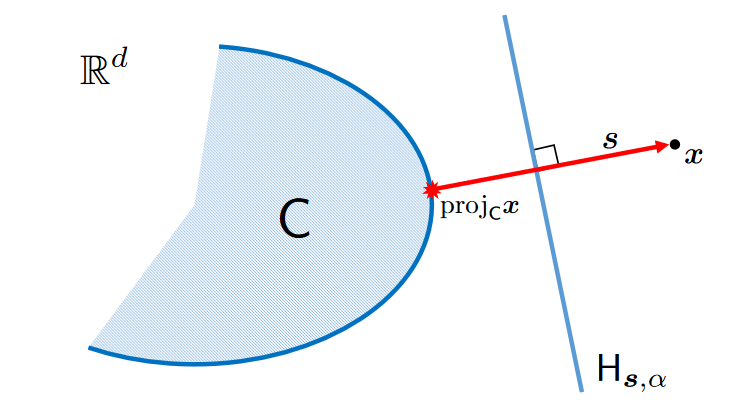
\includegraphics[scale = 0.4]{../images/image4.png}
        \caption{Separating hyperplane between $C$ and $x$}
    \end{center}
\end{figure}

\begin{defn}
    Let $K \subset \RR^n$ be a convex body and $H$ a hyperplane. If $H \cap K \neq \emptyset$ and $K \subset H^+$ or $K \subset H^-$, we call $H$ a \textbf{supporting hyperplane} of $K$ and the corresponding half-space containing $K$ a \textbf{supporting half-space}.
\end{defn}

In the following problem, you will prove that you can always (strongly) separate a point outside of closed convex subset from the closed convex subset. 
\begin{prob}[30 points]
    In this problem, you will prove two separation results. 
\begin{enumerate}[label = (\alph*)]
    \item (10 points) Let $K \subset \RR^n$ be closed and convex. Let $x \in \RR^n$ be an arbitrary point not contained in $K$. Prove that there is a hyperplane $H$ which strongly separates $x$ and $K$.
    \item (20 points) Let $C \subset \RR^n$ be a non-empty closed convex set. For each $x \in \partial C$, there is a hyperplane $H$ such that $C \subset H^-$ and $x \in C \cap H$. 
\end{enumerate} 
\end{prob}

If we are only intersected in separation, then we have the following result which you may assume without proof. 

\begin{thm}
    Let $K, L \subset \RR^d$ be non-empty convex sets satisfying $\rint K \cap \rint L = \emptyset$. Then we can separate $K$ and $L$. 
\end{thm}

\subsection{Facial Structure of Convex Bodies}

In Definition~\ref{definition-height-function}, we define an important function that allows us to describe the geometry of a convex body. 

\begin{defn}\label{definition-height-function}
    For any subset $K \subset \RR^n$, define the \textbf{height function} $h_K : S^{n-1} \to \RR$ defined by 
    \[
        h_K(u) = \sup_{x \in K} \langle x, u \rangle.
    \] 
\end{defn}

Geometrically, the value $h_K(u)$ is the distance of the furthest point on $K$ in the direction of $u$.

\begin{prob} [20 points] \label{problem-height-function}
    Let $K \in \mathsf{K}^n$ body and $u \in S^{n-1}$.
    \begin{enumerate}[label = (\alph*)]
        \item (5 points) Show that there exists $x \in K$ such that $\langle x, u \rangle = h_K(u)$. 
        \item (5 points) Prove that $H = \{x \in \RR^n : \langle x, u \rangle = h_K(u)\}$ is a supporting hyperplane of $K$.
        \item (10 points) If $K, L$ are convex bodies and $a > 0$, then $h_{aL + K} (u) = a h_L(u) + h_K(u)$ for all $u \in S^{n-1}$.
    \end{enumerate}
\end{prob}

We now want to formalize the notion of a ``face" of a convex body. Consider the case of a solid cube $[0, 1]^3 \subset \RR^3$. The common knowledge about the cube is that there are six faces: the six squares. These faces can be viewed as the points which are the furthest in one of the following six directions: $(\pm 1, 0, 0), (0, \pm 1, 0)$, and $(0, 0, \pm 1)$. This motivates Definition~\ref{definition-face}.

\begin{defn} \label{definition-face}
    For any subset $K \subset \RR^n$, we define a \textbf{face} of $K$ to be the intersection of $K$ with any supporting hyperplane. For $0 \leq k \leq \dim K$, a \textbf{k-face} is a face of dimension $k$. We call a face of $K$ a \textbf{facet} if it has dimension $\dim K - 1$. By convention, we let $K$ be a $\dim K$ face of $K$ even if there is not necessarily a supporting hyperplane which makes it so. Define the face of $K$ in the direction of $u \in S^{n-1}$ as
    \[
        F(K, u) := F_K(u) := \{ x \in K : \langle x, u \rangle = h_K(u) \}. 
    \]
\end{defn}
 
Note that from Definition~\ref{definition-face} the cube has more than the six faces described. The faces described consist of all the facets, but all of the ``edges" and ``vertices" will also be faces as well. From Problem~\ref{problem-height-function}, it is not difficult to prove Proposition~\ref{proposition-face-addition}. You may take this result for granted. 

\begin{prop} \label{proposition-face-addition}
    Let $K_1, \ldots,  K_m \subset \RR^n$ be convex bodies and $\alpha_1, \ldots, \alpha_m > 0$. Let $K = \alpha_1 K_1 + \ldots + \alpha_m K_m$. Then 
    \[
        F(K, u) = \sum_{k = 1}^n \alpha_i F(K_i, u).  
    \]
\end{prop}

\begin{defn}
    For a convex body $K \subset \RR^n$, a point $v \in K$ is called a \textbf{vertex} of $K$ if $\frac{1}{2}(y + z) = v$ for $y, z \in K$ implies that $y = z = v$. We denote the set of vertices of $K$ as $v(K)$. 
\end{defn}

The set of vertices $v(K)$ contains all the information we need to determine $K$. This is summarized by Theorem~\ref{vertices-convex-hull} which you may take for granted. 
\begin{thm} \label{vertices-convex-hull}
    Let $K \in \mathsf{K}^n$. Then $K = \conv v(K)$. 
\end{thm} 
Problem~\ref{problem-caratheodory} will imply that you do not need too many of the vertices to specify an arbitrary point in your convex body.
\begin{prob} [15 points] \label{problem-caratheodory}
    Let $S \subset \RR^n$ be an arbitrary subset of vectors. Let $x \in \conv S$. Prove that $x$ can be written as a convex combination of at most $n+1$ elements in $S$. 
\end{prob}

\subsection{Polytopes and Polyhedra}

In this section, we consider two special classes of convex sets: polytopes and polyhedra. These are higher-dimensional generalizations of polygons. 

\begin{defn}
    A \textbf{polytope} is a convex hull of a finite number of points. A \textbf{polyhedra} is the intersection of a finite number of closed half-spaces. Let $\mathsf{P}^n$ denote the family of polytopes in $\RR^n$.
\end{defn}

In general, the set of polytopes and polyhedra are not equivalent. Indeed, polytopes are necessarily bounded while polyhedra may not be. However, in Problem~\ref{problem-weyl-minkowski} you will show that the two concepts are equivalent if we assume boundedness. To aid you in the proof, we introduce a useful duality tool to go from polytopes to polyhedra and vice versa.  

\begin{defn}
    If $K$ is a convex body, define the \textbf{dual} of $K$ as
    \[
        K^\circ := \{ x \in \RR^n : \langle x, p \rangle \leq 1 \text{ for all } p \in K\}.
    \]
\end{defn}
\begin{prob}[20 points]
    Let $K$ be a convex body with $0 \in \tint K$. 
    \begin{enumerate}[label = (\alph*)]
        \item (10 points) Prove that $K^\circ$ is a convex body with $0 \in \tint K^\circ$. 
        \item (10 points) Prove that $K = K^{\circ \circ}$. 
    \end{enumerate}
    In other words, $\cdot^{\circ}$ is a notion of duality on the convex bodies containing $0$ in their interior. 
\end{prob}

\begin{prob} [40 points]\label{problem-weyl-minkowski}
    Let $K \subset \RR^n$ be bounded. In this problem you will prove that $K$ is a polyhedron if and only if it is a polytope. 
    \begin{enumerate}[label = (\alph*)]
        \item (15 points) Suppose that $K = \bigcap_{i = 1}^m H_{n_i, \alpha_i}^-$ is a polyhedron where $H_{n_i, \alpha_i}^- = \{x \in \RR^n : \langle x, n_i \rangle \leq \alpha_i\}$. For $x \in K$, define $\mathsf{ind}(x) = \{i \in [m] : \langle x, n_i \rangle = \alpha_i\}$ to be the indices of the hyperplanes that contain $x$. Prove that if $x \in v(K)$ then $\lin_{i \in \mathsf{ind}(x)} \{n_i\} = \RR^n$. 
        
        \item (10 points) Prove that the number of vertices is finite and conclude that bounded polyhedra are polytopes. 
        
        \item (15 points) Suppose that $K = \conv \{x_1, ..., x_m\} \subset \RR^n$ is a polytope. Prove that
        \[
            K^\circ = \{x \in \RR^n : \langle x, x_j \rangle \leq 1 \text{ for } 1 \leq j \leq m\}.
        \]
        Conclude that polytopes are polyhedra.
    \end{enumerate}
\end{prob}

\subsection{More on the Facial Structure of Convex Bodies}

You may have noticed that there is a discrepancy between the notion of a face and a vertex. We defined a face as the intersection of our convex body with a supporting hyperplane. Thus, faces are defined from the ``outside" of the convex body. On the other hand, we defined vertices from the ``inside" by letting them be the points which cannot be written as a non-trivial convex combination of points in our convex body. If we were to try to define faces more intrinsically, we would make the following formal definition. 

\begin{defn}
    Let $K \in \mathsf{K}^n$. A closed, convex set $F \subset K$ is called a \textbf{feature} of $K$ if whenever $y, z \in K$ and $\frac{1}{2}(y + z) \in F$ then $y, z \in F$. When $k = \dim F$, we call $F$ a \textbf{$k$-feature}. In particular, vertices are $0$-features. We let $\mathcal{F}_i := \mathcal{F}_i(K)$ for $0 \leq i \leq \dim K$ be the collection of $i$-features of $K$. 
\end{defn}

Faces are clearly features, but features are not necessarily faces. Figure~\ref{weird} demonstrates why this is the case. The labelled point is a vertex (0-feature) but not a 0-face. Thus the result Problem~\ref{problem-caratheodory} would not hold if we replaced $v(K)$ with the set of $0$-faces. Hence, features are better than faces at representing information about our convex bodies. Indeed, in the following problem, you will prove that our convex bodies can be partitioned into the relative interiors of our faces. 

\begin{figure}[h]
    \begin{center}
        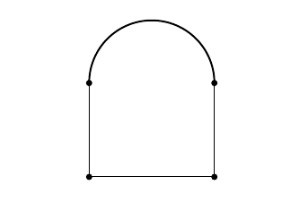
\includegraphics[scale = 1]{../images/image5.png}
        \caption{The top two dotted points are $0$-features but not $0$ faces}
        \label{weird}
    \end{center}
\end{figure}
 
\begin{prob}[15 points]
    Let $\mathcal{F}$ be the collection of all of the features of $K$. Prove that 
    \[
        K = \bigsqcup_{F \in \mathcal{F}} \rint (F).
    \]
    where the union is disjoint. 
\end{prob}

In the case of polytopes, it turns out that features and faces are the exact same concept! This result, along with many other useful properties of features and facets of polytopes, is summarized in Proposition~\ref{proposition-features-faces-polytopes}. You may take these results for granted.  
\begin{prop} \label{proposition-features-faces-polytopes}
    Let $P = \conv \{x_1, ..., x_m\}$ be a polytope in $\RR^n$. 
    \begin{enumerate}[label = (\alph*)] 
        \item If $F$ is a face of $P$, then $F = \conv_{i : x_i \in F} \{x_i\}$. 
        \item If $F$ is a face of $P$ and $F'$ is a face of $F$, then $F'$ is a face of $P$. 
        \item $F \subset P$ is a feature of $P$ if and only if it is a face. 
        \item Let $P \in \mathsf{P}^n$ have full dimension. Let $F_1, \ldots, F_k$ be the facets of $P$ and let $H_1, \ldots, H_k$ be the hyperplanes spanned by the facets such that $P \subset H_i^-$. Prove that 
        \[
            P = H_1^- \cap \ldots \cap H_k^-.
        \]
        \item Let $F_j$ be a $j$ face and $F_k$ be a $k$ face of the polytope $P$ which satisfy $F_j \subset F_k$. Then for each $j+1 \leq i \leq k-1$, there exists $F_i \in \mathcal{F}_i(P)$ such that 
        \[
            F_j \subset F_{j+1} \subset \ldots \subset F_{k-1} \subset F_k.
        \]
    \end{enumerate}
\end{prop}

\subsection{Volume of Convex Bodies}

The $n$-dimensional \textbf{volume} of a convex body $K \subset \RR^n$, which we write as $\Vol_n(K)$ is a measurement of the size of $K$. The volume is a well-defined concept for convex bodies and can be defined via an integral over $\RR^n$. Indeed, the volume of a convex body $E \subset \RR^n$ (or in general any Lebesgue measurable set) is equal to the integral
\[
    \Vol_n(E) := \int_{\RR^n} \1_E \, d\lambda 
\] 
where the integral is taken with respect to the Lebesgue measure $\lambda$ on $\RR^n$. However, for this power round, you will not need to know measure theory or invoke any integrals. In a later problem, you will prove an inductive formula for the volume of polytopes which will suffice for our purposes. In order to avoid the use of calculus, you may black box the following result. 

\begin{prop} \label{volume-properties}
    The volume operator enjoys the following properties:
    \begin{enumerate}[label = (\alph*)]
        \item For $K \in \mathsf{K}^n$ and $\lambda \geq 0$, $\Vol_n(\lambda K) = \lambda^n \Vol_n (K)$. 

        \item For convex bodies $L \subset K \subset \RR^n$, $0 \leq \Vol_n(L) \leq \Vol_n(K)$.

        \item $\Vol_n(T(K) + v) = |\det T| \cdot \Vol_n(K)$ where $v \in \RR^n$ and $T : \RR^n \to \RR^n$ is a linear map. In particular, rigid motions preserve volume. 

        \item $\Vol_n(Q_n) = 1$ where $Q_n$ is the unit cube. 

        \item Let $K \subset \RR^{n-1}$ be a convex body and let $z = x \times \{h\} \in \RR^{n-1} \times \RR = \RR^n$ with $h \neq 0$. Then $\Vol_n(\conv \{K \times \{0\}, z\}) = \frac{1}{n} \cdot \Vol_{n-1}(K) \cdot |h|$. 
    \end{enumerate}
\end{prop}

\begin{remark}
    Note that in each dimension, we have a separate volume operator which can assign different volumes to different convex bodies. For example, a unit square in $\RR^2$ will have $2$-dimensional volume of $1$ and a $3$-dimensional volume of $0$. Property (e) of Proposition~\ref{volume-properties} gives the formula for computing pyramids. 
\end{remark}

Another way to define volume is to partition your object into subobjects whose volume you know how to calculate. In the following problem, you will explore this approach by proving that you are able to nicely approximate open sets. The problem asks you to work in $\RR^2$, but the result holds for any $\RR^n$. 

\begin{prob}[20 points]
    Let $K$ be a convex body with non-empty interior $\tint K = \mcO \subset \RR^2$. The set $\mathcal{O}$, by definition, is open. Prove that there exists a sequence set of closed cells $R_1, R_2, \ldots$ such that 
    \[
        \mathcal{O} = \bigcup_{n \geq 1} R_n
    \]
    where $R_n \cap R_m \subset \partial R_n \cap \partial R_m$ for all $m \neq n$ and for any $\varepsilon > 0$, there is a large enough $N > 0$ such that 
    \[
        \varepsilon B^2 + \bigcup_{n = 1}^N R_n \supset K.
    \]
    A closed cell in $\RR^2$ is a set of the form $[a, b] \times [c, d]$ where $a \leq b$ and $c \leq d$.

\end{prob}

The condition $R_n \cap R_m \subset \partial R_n \cap \partial R_m$ means that $R_n$ and $R_m$ intersect on their boundary, which has no two-dimensional volume. After approximating an open set in this way, we can possibly define our volume as 
\[
    \Vol_2(\mathcal{O}) = \sum_{n = 1}^\infty \Vol_2(R_n).    
\]
The volumes of our cells $R_n$ are easy to calculate simply by multiplying the side lengths. Note that in order to define volume in this way, it remains to show that the sum does not depend on the choice of approximation $\{R_n\}_{n \geq 1}$. This is indeed the case, but we will not require you to prove it. After defining volume for open sets, another possible way we could define the volume of a convex body (with non-empty interior) is 
\[
    \Vol_d(K) := \Vol_d(\tint K).    
\]

\begin{prob} [30 points] \label{computing-volumes}
     In this problem, you will compute some volumes. 
    \begin{enumerate}[label = (\alph*)]
        \item (10 points) Find the value of the volume of the tetrahedron
        \[
            \Vol_n \left ( \left \{ (x_1, \ldots, x_n) \in \RR^n : 0 \leq x_1 \leq \ldots \leq x_n \leq 1 \right \} \right ).    
        \]
        \item (10 points) Find the value of the volume of the unit $\norm{\cdot}_1$ ball
        \[
            \Vol_n \left ( \left \{ x \in \RR^n : \norm{x}_1 = \sum_{k = 1}^n |x_k| \leq 1 \right \} \right ).
        \]
        
        \item (10 points) Given $m$ vectors $\mathcal{V} := \{v_1, \ldots, v_m \} \subset \RR^n$, define the \textbf{zonotope}
        \[
            Z(\mathcal{V}) := \left \{ \sum_{i = 1}^m \lambda_i v_i : \lambda_i \in [0, 1] \text{ for all } 1 \leq i \leq m \right \}.
        \]
        Let $\mathcal{B} = \{v_1, \ldots, v_n\}$ be $n$ vectors in $\RR^n$. Prove that 
        \[
            \Vol_n(Z(\mathcal{B})) = | D(v_1, \ldots, v_n) |.
        \]
    \end{enumerate}
\end{prob}

\begin{prob} [25 points] \label{inductive-volume}
    Let $K \subset \mathsf{P}^n$ with $\dim K = n$. Let $F_1, \ldots, F_N$ be the facets of $K$ with unit normals $u_1, \ldots, u_N$.
    \begin{enumerate}[label = (\alph*)]
        \item (15 points) Prove that 
        \[
            \sum_{i = 1}^N \Vol_{n-1}(F_i) \cdot \langle u_i, z \rangle = 0
        \]
        for all $z \in \RR^n$. 

        \item (10 points) Prove that 
        \[
            \Vol_n(K) = \sum_{i = 1}^N \frac{1}{n} \cdot \Vol_{n-1}(F_i) \cdot h_K(u_i)
        \]
    \end{enumerate}
\end{prob}




\subsection{Hausdorff Distance}

It is difficult to work with generic convex bodies because of their variety. In this section, we show that there is a metric that we can put on the space of compact subsets (in particular, convex bodies) which allows us to introduce continuity to the relevant area measures we are using. This will also allow us to approximate our convex bodies with nice families of polytopes to make our computations more straightforward and combinatorial.

To this end, we define a metric on the space $\mathsf{K}^n$ which we call the Hausdorff distance or Hausdorff metric. Geometrically, the Hausdorff distance is the smallest thickening we need so that the thickening of each one contains the other. 

\begin{defn} \label{definition-hausdorff-distance}
    We call the function $\delta : \mathsf{C}^n \times \mathsf{C}^n \to \RR_{\geq 0}$ defined by
\begin{align*}
    \delta(K, L) & = \max \left \{ \sup_{x \in K} \inf_{y \in L} |x-y|, \sup_{y \in L} \inf_{x \in K} |x-y| \right \} \\
    & = \inf \{\varepsilon \geq 0 : K \subset L + \varepsilon B^n, L \subset K + \varepsilon B^n\} 
\end{align*}
    the \textbf{Hausdorff distance} or \textbf{Hausdorff metric}. Hence, the number $\delta(K, L)$ will be the Hausdorff distance between $K$ and $L$. 
\end{defn}

The equivalence in Definition~\ref{definition-hausdorff-distance} is not immediately clear, but it is not difficult to prove. You may take the equivalence for granted. In the next problem, you will prove more properties of the Hausdorff distance. In particular, you will prove that it is indeed a metric on the space of compact subsets. For convenience, we will define $\mathsf{C}^n$ to be the space of non-empty compact subsets of $\RR^n$. 

\begin{prob}[15 points]
    Let $K$ and $L$ be compact subsets of $\RR^n$. 
    \begin{enumerate}[label = (\alph*)]
        \item (10 points) Prove that if $\varepsilon = \delta(K, L)$, then $K \subset L + \varepsilon B^n$ and $L \subset K + \varepsilon B^n$.  

        \item (5 points) Prove that $\delta$ is a metric on $\mathsf{C}^n$. 
    \end{enumerate}
\end{prob}


In the next problem, you will prove that $\mathsf{P}^n$ is dense in $\mathsf{K}^n$ with respect to the Hausdorff metric. This will allow you to compute continuous functions defined on the convex bodies by approximating an arbitrary body by polytopes. In many situations, the value of a continuous functions on $\mathsf{K}^n$ will be easier to calculate on $\mathsf{P}^n$. 
 
\begin{prob} [20 points]
    Let $C \in \mathsf{K}^n$ be a convex body. For any $\varepsilon > 0$, there exists a polytope $C_\varepsilon \in \mathsf{P}^n$ such that $\delta (C, C_\epsilon) < \epsilon$. 
\end{prob} 

\begin{remark}
    Most of the functions that we have worked with so far are continuous on $\mathsf{K}^n$ when we consider $\mathsf{K}^n$ as a metric space equipped with the Hausdorff metric. In particular, the projection operator $\mathsf{proj}_x : \mathsf{K}^n \to \RR^n$ defined by $\mathsf{proj}_x(K) = \pi_K(x)$, the distance operator $\mathsf{dist}_x : \mathsf{K}^n \to \RR$ defined by $\mathsf{dist}_x(K) = \dist(x, K)$, and the volume operator $\Vol_n(\cdot)$ are continuous. You may take this fact for granted. 
\end{remark}

The following problems will be centered around the metric space $(\mathsf{C}^n, \delta)$.

\begin{prob} [20 points]
    Prove that the metric space $(\mathsf{C}^n, \delta)$ is complete. Hint: Let $\{K_n\}_{n \geq 1} \subset \mathsf{C}^n$ be a Cauchy sequence and consider the set $K := \bigcap_{m \geq 1} \clo \left ( \bigcup_{j \geq m} K_j \right ).$
\end{prob}


In Problem~\ref{problem-IFS}, this metric space becomes a useful tool in determining the uniqueness of certain fractals which arise as limit sets of dynamical systems. This is unrelated to the theory of convex bodies, but it is an interesting application of Hausdorff distance. 

\begin{figure}[h]
\begin{center}
    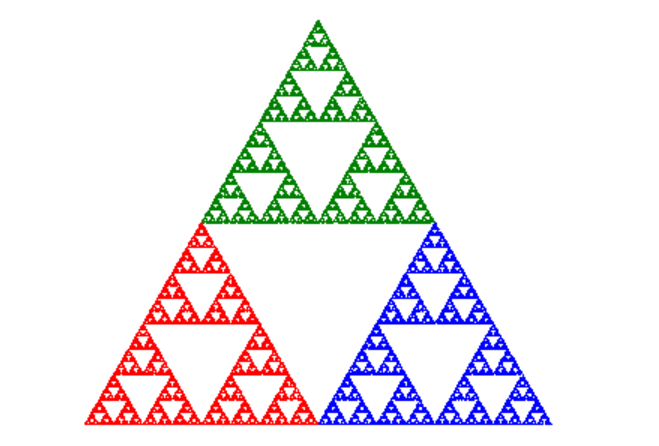
\includegraphics[scale = 0.4]{../images/image6.png}
    \caption{The red, blue, green correspond to the images of $f_1, f_2, f_3$, respectively.}
    \label{sierpinski}
\end{center}
\end{figure}

\begin{prob}[Limit Sets of Dynamical Systems, 60 points] \label{problem-IFS}
    Let $C \subset \RR^n$ be a closed set. Let $f_1, \ldots, f_m : C \to C$ be maps such that $|f_i(x) - f_i(y)| \leq c_i |x-y|$ where $c_i \in (0, 1)$ for all $1 \leq i \leq m$ and $x, y \in C$. 
    \begin{enumerate}[label = (\alph*)]
        \item (30 points) Prove that there is a unique non-empty compact set $K \subset \RR^n$ such that $K = f_1(K) \cup \ldots \cup f_m(K)$. 
        \item (30 points) Let $K$ be the compact set from (a). Prove that if $E \subset C$ is a compact subset satisfying $f_i(E) \subset E$ for all $1 \leq i \leq m$, then 
        \[
            K = \bigcap_{i \geq 0} \left \{ \bigcup_{j_1, \ldots, j_i \in [m]} (f_{j_1} \circ \ldots \circ f_{j_i})(E) \right \}.
        \]
    \end{enumerate}
\end{prob}

Problem~\ref{problem-IFS} gives the existence of certain limit sets of dynamical systems. For example, it gives the existence of the Sierpinski gasket for the dynamical system defined by the homotheties
    \begin{align*}
        f_1(x, y):= \left ( x/2, y/2 \right ), \quad f_2(x, y):= \left ( (x+1)/2, y/2 \right ), \quad f_3(x, y) := \left ( (x+1)/2, y/2 + \sqrt{3}/4 \right ) 
    \end{align*}
    as shown in Figure~\ref{sierpinski}. Similarly, you can find dynamical systems which give other famous self-similar fractals, such as the Koch Snowflake, Sierpinski carpet, etc., as their limit set.



\newpage

\section{Introduction to Mixed Volumes}

Let $K_1, \ldots, K_m$ be convex bodies in $\RR^n$. In the section, we will be interested in the value of $\Vol_n (K_1 + \ldots + K_m)$. Even more generally, we can attach dilation factors $\lambda_i > 0$ and consider the function $\Vol_n \left ( \sum_{i = 1}^n \lambda_i K_i \right )$ in $n$ variables. What is the behavior of this expression in terms of $\lambda_1, \ldots, \lambda_n$? We begin with an example $P, B\subset \RR^2$ where $P$ is some polygon and $B$ is the unit ball. 

\begin{figure}[h]
\begin{center}
    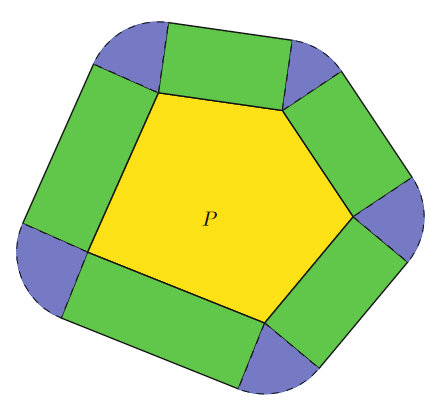
\includegraphics[scale = 0.7]{../images/image7.png}
    \caption{The sum of $P$ and the unit ball $B$}
    \label{minkowski-sum-example}
\end{center}
\end{figure}

The sum of $P$ and $Q$ is shown in Figure~\ref{minkowski-sum-example}. In the diagram, we have partitioned the sum into three regions: yellow, green, and blue. The area of the yellow region is exactly the area of $P$. The area of the green region is exactly the perimeter of $P$ multiplied by the radius of $B$. You can also convince yourself that the area of the blue region is the area of $B$. This gives us the formula:
\[
    \Vol_2(P+B) = \Vol_2(P) + \per(P) + \Vol_2(B).
\]
Now, adding weights $\lambda$ and $\mu$ to $P$ and $B$, respectively, we can generalize our formula to  
\[
    \Vol_2( \lambda P + \mu B) = \lambda^2 \cdot \Vol_2(P) + \lambda \mu \cdot \per (P) + \mu^2 \cdot \Vol_2(B).
\]
One observation is that this formula is a homogeneous polynomial of degree $2$. Another observation is that the coefficients are all positive valued and seem to involve different types of ``intrinsic" geometric measures of our convex bodies. It is reasonable to ask whether or not these two trends holds in arbitrary dimension with an arbitrary number of convex bodies in the sum. Indeed, this pattern does hold where the corresponding coefficients are encapsulated by the multivariate function $V : (\mathsf{K}^n)^n \to \RR_{\geq 0}$ which we call the \textbf{mixed volume}. To define the mixed volume, we need the convex bodies to be in the same space $\RR^n$ and the number of convex bodies it takes is the dimension of the ambient space. The goal of this section is for you to prove Theorem~\ref{minkowski-theorem}. 
\begin{thm}\label{minkowski-theorem}
    There is a non-negative symmetric function $V : (\mathsf{K}^n)^n \to \RR$ such that for all $C_1, ..., C_m \in \mathsf{K}^n$ such that for all $\lambda_1, ..., \lambda_m \geq 0$ we have that
    \[
        \Vol_n(\lambda_1 C_1 + ... + \lambda_m C_m) = \sum_{i_1, ..., i_n = 1}^m V(C_{i_1}, ..., C_{i_n}) \lambda_{i_1} ... \lambda_{i_n}. 
    \]
\end{thm}

\subsection{Mixed Volume Formula for Polytopes}

We first prove the theorem for polytopes. Recall from Problem~\ref{inductive-volume} the following inductive formula for the volume of a polytope $P \in \mathsf{P}^n$.  
\begin{prop}
    Let $P \subset \mathsf{K}^n$ be a $n$-dimensional polytope and let $\mathcal{U}$ be the set of unit vectors normal to the facets. Then
    \[
        \Vol_n(P) = \frac{1}{n} \sum_{u \in \mathcal{U}} h_P(u) \cdot \Vol_{n-1} (F_P(u)).
    \]
\end{prop}

Assuming we want a theorem like Theorem~\ref{minkowski-theorem} to hold, substituting our expression $\lambda_1 C_1 + \ldots + \lambda_m C_m$ into $P$ only gives us a few possibilities. However, one possible problem is that the set of unit vectors $\mathcal{U}$ is dependent on $P$ and might change depending on the $\lambda_i$'s. Luckily, Problem~\ref{problem-addition} shows that this is not the case. 

\begin{prob} [15 points] \label{problem-addition}
    Let $P_1, \ldots, P_m \in \mathsf{P}^n$ be polytopes in $\RR^n$. Let $P = P_1 + \ldots + P_m$ and $P_\lambda = \lambda_1 P_1 + \ldots + \lambda_m P_m$. Prove that $\dim F_P(u) = \dim F_{P_\lambda}(u)$ whenever $\lambda_1, \ldots, \lambda_m > 0$. In particular, as long as $\lambda_1, \ldots, \lambda_m > 0$, the facet unit normals will remain the same.  
\end{prob}

This motivates the following definition of the mixed volume. 

\begin{defn}
    Let $P_1, \ldots, P_n \in \mathsf{P}^n$ be polytopes and let $\mathcal{U}$ be the set of unit facet normals of $P_1 + \ldots + P_{n-1}$. We define their mixed volume $V (P_1, \ldots, P_n) := V_n (P_1, \ldots, P_n)$ inductively by 
    \[
        V_n (P_1, \ldots, P_n) = \frac{1}{n} \sum_{u \in \mathcal{U}} h_{P_n} (u) \cdot V_{n-1}(F_{P_1}(u), \ldots, F_{P_{n-1}}(u))
    \]  
    for $n \geq 2$ where we view the $F_{P_i}(u)$'s on the right hand side as convex bodies in $\RR^{n-1}$ by projecting them onto the hyperplane perpendicular to $u$ passing through $0$. To make this distinction clear, we sometimes denote this by $F_{P_i}(u)|_{u^\perp}$. For $n = 1$ and $P_1 = [a, b]$, we define $V_1(P_1) := b-a$. 
\end{defn}

Given this definition of the mixed volume, we can now prove the main theorem. 

\begin{prob} [30 points]
    Prove Theorem~\ref{minkowski-theorem} for polytopes. That is, prove that for polytopes $P_1, \ldots, P_m \in \mathsf{P}^n$ and non-negative scalars $\lambda_1, \ldots, \lambda_m \geq 0$ that the following identity holds:
    \[
        \Vol_n(\lambda_1 P_1 + \ldots + \lambda_m P_m) = \sum_{i_1, \ldots, i_n = 1}^m V(P_{i_1}, \ldots, P_{i_n}) \cdot \lambda_{i_1} \ldots \lambda_{i_n}.
    \]   
\end{prob}

\subsection{Extending the Mixed Volume to Arbitrary Convex Bodies}

So far, we have only defined the mixed volume on polytopes. In this section, we try to extend this to general convex bodies. In the next problem, you prove that you can extend the definition of the mixed volume to collections of general convex bodies by approximating the convex bodies with polytopes and taking the limit.

\begin{prob} [50 points] \label{problem-extending-mixed-volumes}
    Let $K_1, \ldots, K_n \in \mathsf{K}^n$ be convex bodies in $\RR^n$. For all $i \in [n]$, let $(P_i^{(j)})_{j \geq 1}$ be a sequence of polytopes converging to $K_i$ with respect to the Hausdorff distance. 
    \begin{enumerate}[label = (\alph*)]
        \item (20 points) Let $P_1, \ldots, P_n \in \mathsf{P}^n$. Then, prove that 
        \[
            V(P_1, \ldots, P_n) = \frac{1}{n!} \sum_{I \subset [n]} (-1)^{n + |I|} \cdot \Vol_n \left ( \sum_{i \in I} P_i \right ).
        \]  
        \item (10 points) Prove that the sequence $V_n(P_1^{(j)}, \ldots, P_n^{(j)})$ is convergent and that the limit is independent of the choice of our approximating sequences of polytopes. We define $V(K_1, \ldots, K_n) = \lim_{j \to \infty} V_n(P_1^{(j)}, \ldots, P_n^{(j)})$ to be the mixed volume of $K_1, \ldots, K_n$. 
        
        \item (15 points) Prove that Theorem~\ref{minkowski-theorem} holds for general convex bodies. 
        
        \item (5 points) Prove that the mixed volume $V_n : (\mathsf{K}^n)^n \to \RR_{\geq 0}$ is a continuous function. 
    \end{enumerate}
\end{prob}

From Problem~\ref{problem-extending-mixed-volumes}, you can conclude that the mixed volume, when computed on general convex bodies, satisfies the same properties as in Problem~\ref{some-properties}. Note that Problem~\ref{problem-extending-mixed-volumes}(a) immediately implies that the mixed volume is symmetric in its arguments. This allows us to derive yet another formula for the mixed volume given by 
\[
    V_n(P_1, \ldots, P_n) = \frac{1}{n!} \frac{\partial^n}{\partial x_1 \ldots \partial x_n} \Vol_n(x_1 P_1 + \ldots + x_n P_n). 
\]
This is left as an exercise to the interested reader. 
\subsection{Properties of Mixed Volumes}
We now explore a few properties of mixed volumes. 

\begin{prob} [35 points] \label{some-properties}
    Let $P_1, \ldots, P_n \in \mathsf{P}^n$ be polytopes in $\RR^n$. 
    \begin{enumerate}[label = (\alph*)]
        \item (10 points) For any vector $v \in \RR^n$ and linear map $A : \RR^n \to \RR^n$, we have that  
        \begin{align*}
            V(P_1 + v, \ldots, P_n) = V(P_1, \ldots, P_n) \text{ and } V(A(P_1), \ldots, A(P_n)) = |\det A| \cdot V(P_1, \ldots, P_n).
        \end{align*}
        
        \item (10 points) The mixed volume is linear in each argument with respect to set addition and non-negative dilations. That is, for $P_1^{(1)}, P_1^{(2)} \in \mathsf{P}^n$ and $a > 0$, we have that 
        \begin{align*}
            V_n(a \cdot P_1^{(1)} + P_1^{(2)}, P_2, \ldots, P_n) & = a \cdot V_n(P_1^{(1)}, P_2, \ldots, P_n) + V_n(P_1^{(2)}, P_2, \ldots, P_n).
        \end{align*}

        \item (15 points) Prove that for $P_1, \ldots, P_n, Q_1, \ldots, Q_n \in \mathsf{K}^n$ with $P_i \subset Q_i$ for all $1 \leq i \leq n$, we have that 
        \[
            0 \leq V(P_1, \ldots, P_n) \leq V(Q_1, \ldots, Q_n).
        \]
    \end{enumerate}
\end{prob}

Problem~\ref{some-properties} implies that the mixed volumes enjoys many of the properties of $\Vol_d$. Indeed, the mixed volume is translation invariant and scales by the determinant of a linear map when that linear map is applied to its argument. The mixed volume is always positive, a property which we would want to be true for a accurate notion of volume. Already, in Problem~\ref{some-properties}, we have seen that the mixed volume has better properties than the volume due to its ``positive''-multilinearity. In Problem~\ref{problem-mixed-volume-properties-final}, the mixed volume will emerge as a generalization of not only the volume, but also surface measures, etc. 
\begin{prob} [35 points] \label{problem-mixed-volume-properties-final}
    The following problems are some more properties of mixed volumes. 
    \begin{enumerate}[label = (\alph*)]
        \item (5 points) Prove that $V(K, \ldots, K) = \Vol_n(K)$. 
        \item (5 points) Let $K, L \in \mathsf{K}^n$. Prove that 
        \[
            \Vol_n(\lambda_1 K + \lambda_2 L) = \sum_{r = 0}^n \binom{n}{r} V(K[r], L[n-r]) \lambda_1^r \lambda_2^{n-r}    
        \]
        where $V(K[r], L[n-r])$ denotes the mixed volume with $r$ copies of $K$ and $n-r$ copies of $L$. 
        \item (10 points) One intuitive way to define the surface area of a convex body $K \subset \RR^n$ is to thicken it by $\varepsilon$ and divide the thickened part by $\varepsilon$. When $\varepsilon \to 0$, the resulting number should morally be the surface area. It turns out for convex bodies, this number exists and can be written in terms of a mixed volume. In particular, prove that  
        \[
            \lim_{N \to \infty} \frac{\Vol_n \left (K + \frac{1}{N} \cdot B^n \right ) - \Vol_n(K)}{1/N} = n V(K[n-1], B^n).
        \]
        \item (15 points) Recall the definition of zonotope in Problem~\ref{computing-volumes}. Let $\mcV = \{v_1, \ldots, v_m\}$ be a collection of vectors in $\RR^n$ where $m \geq n$. Prove that 
        \[
            \Vol_n(Z(\mcV)) = \sum_{I \subset \mcV : |I| = n} \Vol_n(Z(I)).
        \] 
    \end{enumerate}
\end{prob}

\newpage 

\section{An Inequality about Mixed Volumes}

\subsection{Isoperimetric Inequalities}

In this section, we explore a beautiful inequality at the heart of convex geometry. As applications, you will see that it is a generalization of the isoperimetric inequality and has manifold appearances in different areas of math including combinatorics and algebraic geometry. The inequality is given in the following theorem. 

\begin{thm} \label{alexandrov-fenchel}
    For convex bodies $K, L \in \mathsf{K}^n$ and any fixed collection $(C_1, ..., C_{n-2}) \in (\mathsf{K}^n)^{n-2}$ we have that
    \[
        V(K, L, C_1, ..., C_{n-2})^2 \geq V(K, K, C_1, ..., C_{n-2}) V(L, L, C_1, ..., C_{n-2})
    \]
\end{thm}

In the following problems, you will see the many consequences of this inequality. 

\begin{prob} [40 points]
    Prove the following inequalities. 
    \begin{enumerate}[label = (\alph*)]
        \item (35 points) Prove that for any $1 \leq r \leq n$, we have 
        \[
            V(K_1, \ldots, K_n)^r \geq V(K_1[r], \mcP_r) \cdot \ldots \cdot V(K_r[r], \mcP_r)
        \]
        where $\mcP_r = \{K_{r+1}, \ldots, K_n\}$. 
        \item (5 points) Prove that $V(K_1, \ldots, K_n)^n \geq \Vol_n(K_1) \ldots \Vol_n(K_n)$
    \end{enumerate}
\end{prob}

Before attempting to prove Theorem~\ref{alexandrov-fenchel}, there are still a few tools we must introduce that will help streamline the proof.
\subsection{Simple Consonant Polytopes}

In the next section, it will be useful to have access to a family of approximating polytopes that have a well-understood facial structure. In this way, we can reduce many problems about mixed volumes to combinatorics (and linear algebra). The goal of this section will be to prove another polytope approximation theorem with a smaller collection of polytopes. This collection will enforce a uniform collection of unit facet normals and a symmetry on the adjacencies of facets. 

\begin{defn}
    A polytope $P \in \mathsf{P}^n$ is called \textbf{simple} if every vertex is contained in $n$ facets. 
\end{defn}

Prototypical examples of simple polytopes are polygons in $\RR^2$ or a tetrahedron in $\RR^3$. Restricting ourselves to simple polytopes will ensure that our polytopes have interior and are facially symmetrical. In particular, if we consider the graph where the vertices are our facets and the edges represent adjacency as facets, then the resulting graph with be a regular graph of degree $n$. The next definition is a slightly stronger notion of having a uniform collection of unit facet normals. 

\begin{defn}
    Two polytopes $P, Q \in \mathsf{P}^n$ are said to be \textbf{consonant} if for every $u \in S^{n-1}$ we have 
    \[
        \dim F(P, u) = \dim F(Q, u).     
    \]
\end{defn}

For examples of consonant polytopes, see Figure~\ref{consonance}. Consonant polytopes satisfy the following two properties. 

\begin{figure}[h]
\begin{center}
    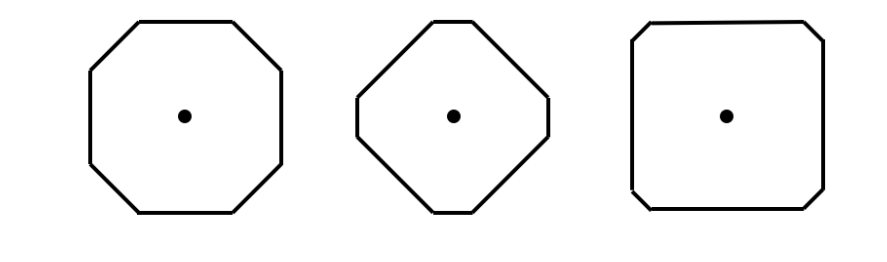
\includegraphics[scale = 0.6]{../images/image8.png}
    \caption{Three consonant polytopes}
    \label{consonance}
\end{center}
\end{figure}
\begin{prop}
    Let $P_1, P_2 \in \mathsf{P}^n$ be polytopes. 
    \begin{enumerate}[label = (\alph*)]
        \item The polytopes $\lambda_1 P_1 + \lambda_2 P_2$ for $\lambda_1, \lambda_2 > 0$ are all consonant to each other. Moreover, if $P_1$ and $P_2$ are consonant, this holds for $\lambda_1, \lambda_2 \geq 0$ where $\lambda_1 + \lambda_2 > 0$. 
        \item If $P_1$ and $P_2$ are consonant, the faces $F(P_1, u)$ and $F(P_2, u)$ are consonant whenever $u \in S^{n-1}$.
        \item If $P$ and $Q$ are consonant and $Q$ is simple, then $P$ is also simple.  
    \end{enumerate}
\end{prop}

To make our study of simple consonant polytopes easier, we introduce another geometric object related to convex bodies called the normal cone. The normal cone always takes a polytope, a face, and a base point in the convex body. Geometrically, the normal cone with respect to a point is the set of vectors $u$ such that the projection of $u + x$ onto the convex body $K$ is $x$. 

\begin{defn}
    For a convex body $K \in \mathsf{K}^n$, define the \textbf{normal cone} of $K$ at $x$ as 
    \[
        N(K, x) := N_K(x) = \{u \in \RR^n : \langle x, u \rangle = h_K(u) \}.    
    \]
\end{defn}

In this definition, the convex cone is the set of vectors where $x$ achieves the value of the support function. That is, $x$ is one of the points on $K$ furthest away from the origin in direction $u$. 

\begin{prob} [40 points] \label{normal-cone-properties}
    In this problem, you will prove some properties of the normal cone. 
    \begin{enumerate}[label = (\alph*)]
        \item (10 points) Verify that our geometric intuition about the normal cone is correct. Specifically, prove that $N_K(x) := \{u \in \RR^n : \pi_K(u + x) = x\}$. 
        \item (15 points) Let $K, L \in \mathsf{P}^n$. Prove that $N_{K+L}(x+y) = N_K(x) \cap N_L(y)$ for all $x \in K, y \in L$.
        \item (15 points) Let $K \in \mathsf{P}^n$ and $x, y \in P$ be two points. Prove that $N_K(x) = N_K(y)$ if and only if the smallest faces containing $x$ and $y$ are the same. 
    \end{enumerate}
\end{prob}
From Problem~\ref{normal-cone-properties}(c), we are able to define the normal cone $N_K(F)$ with respect to a face $F \subset K$. This is because the result in the problem implies that the normal cones of the points in the relative interior of $F$ will be the same. In particular, this implies that there is tiling of $\RR^n$ by the normal cones given by the equation:
\[
    \RR^n = \bigsqcup_{F \subseteq P} (\rint F + N_P(F))    
\]
where $P$ is a polytope and the disjoint union is over all faces of $P$. In the union, we also consider $P$ to be a face of $P$. You can check that $N_P(P) = \{0\}$ which accounts for the relative interior of $P$. For polytopes, there is a nice characterization of the normal cone in terms of the unit normals.

\begin{figure}[h]
\begin{center}
    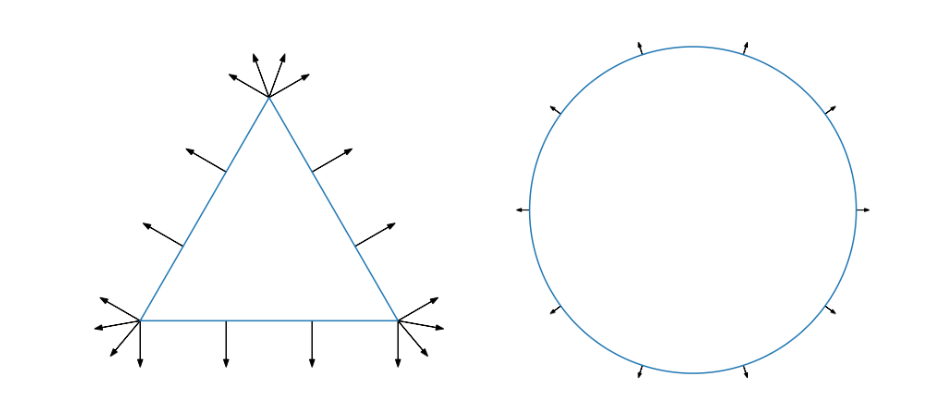
\includegraphics[scale = 0.6]{../images/image9.png}
    \caption{Normal cones of a triangle and a circle}
\end{center}
\end{figure}

\begin{prob} [40 points]
    Let $P = \bigcap_{i = 1}^m H_{u_i, \alpha_i}^-$ be a polyhedron. Recall in Problem~\ref{problem-weyl-minkowski} we defined $\mathsf{ind}(x) = \{i \in [m] : \langle x, u_i \rangle = \alpha_i\}$ to be the indices of the hyperplanes that contain $x$. 
    \begin{enumerate}[label = (\alph*)]
        \item (20 points) Prove that $N_P(x) = \pos \{u_i : i \in \mathsf{ind}(x) \}$.
        \item (20 points) Prove that $\dim F + \dim N_P(F) = n$ whenever $F$ is a face of $P$. 
    \end{enumerate}
\end{prob}

The main idea behind why we are able to pick polytopes that are simple is that ``most polytopes are simple''. We won't formalize this concept, and instead we will just black-box the following result about generating simple polytopes.

\begin{thm}
    Let $P \in \mathsf{P}^n$ be a polytope with non-empty interior and unit facet normals $u_1, \ldots, u_N$. Then, for every $\varepsilon > 0$ there exist reals $\alpha_1, \ldots, \alpha_N$ with $|\alpha_i| \leq \varepsilon$ and 
    \[
        P' := \bigcap_{k = 1}^N H_{u_k, h_P(u_k) + \alpha_i}^-    
    \]
    is a simple polytope with unit facet normals $u_1, \ldots, u_N$. Moreover, for every $x \in v(P')$ there exists $y \in P$ such that $N_{P'}(x) \subseteq N_P(y)$. 
\end{thm}

Thus, given a polytope, we can make arbitrarily small perturbations to make it simple and also satisfy the nice normal cone containment property. The next result connects consonance with the normal cones. 

\begin{prob} [40 points]
    Prove that $P_1, P_2 \in \mathsf{P}^n$ are consonant if and only if 
    \[
        \{N_{P_1}(v) : v \in v(P_1) \} = \{N_{P_2}(v) : v \in v(P_2) \}.   
    \]
\end{prob}

We finally have all the tools to prove the final approximation result. 

\begin{prob} [40 points]
    Let $K_1, \ldots, K_m \in \mathsf{K}^n$ be convex bodies. In this problem, you will prove that for every $\varepsilon > 0$ there exist simple consonant polytopes $P_1, \ldots, P_m \in \mathsf{P}^n$ such that $\delta(K_i, P_i) < \varepsilon$ for $i$, $1 \leq i \leq m$.
\end{prob}

Thus, when we are working with mixed volumes, we can approximate our polytopes with ones which are simple and consonant. Any results in the general case can then be obtained by taking the limit.

\subsection{Extending the Mixed Volume to a Bilinear Form}
In this section, you will see how we can translate the mixed volume to the world of linear algebra. The main idea is that a family of consonant polytopes can be specified by a vector in a finite dimensional vector space. Indeed, let $P \in \mathsf{P}^n$ be a polytope and let 
\[
    [P] := \{Q \in \mathsf{P}^n : \text{$P$ and $Q$ are consonant} \}.
\]
Then, all the polytopes in $[P]$ share unit normal directions $\mathcal{U} = \{u_1, \ldots, u_N\}$. For $1 \leq i \leq N$, we can then define $h_i(Q) = h(Q, u_i)$ for $Q \in [P]$ and $h(Q) := (h_1(Q), \ldots, h_N(Q))$. The polytope $Q$ can then be shown to be equal to 
\[
    Q = \bigcap_{i = 1}^N \{ x \in \RR^n : \langle x, u_i \rangle \leq h_i(Q)\}.    
\]
Hence $h$ induces an injection from $[P]$ into $\RR^N$. 

\begin{prob} [5 points]
    Prove that $h$ embeds $[P]$ into $\RR^N$ as a cone. That is, prove that $h(\lambda \cdot P_1 + P_2) = \lambda \cdot h(P_1) + h(P_2)$ for all $\lambda \geq 0$ and $P_1, P_2 \in [P]$. 
\end{prob}

The next problem will be a key result for future sections. 

\begin{prob} [30 points]
    Let $\mathcal{P} = \{C_1, \ldots, C_{n-2}\} \subset \mathsf{P}^n$ be a fixed collection of simple consonant polytopes in $[P]$. Prove that there exists a graphic matrix $M$ and a diagonal matrix $D$ such that 
    \[
        V(P_1, P_2, \mathcal{P}) = \langle h(P_1), (M-D) h(P_2) \rangle    
    \]
    whenever $P_1, P_2 \in [P]$. A diagonal matrix is a square matrix where the only non-zero terms lie on the main diagonal. 
\end{prob}

This implies that whenever we are restricting the arguments of the mixed volume to polytopes in the same consonant class, we can extend $V( \cdot, \cdot, \mathcal{P})$ to a bilinear form on $\RR^N$ defined by 
\[
    V(x, y, \mathcal{P}) := \langle y, (M-D)x \rangle. 
\]

\subsection{Proof of Theorem~\ref{alexandrov-fenchel}}
In the following problem, you will prove Theorem~\ref{alexandrov-fenchel} for convex bodies in $\RR^2$. 

\begin{prob} [40 points]
    Let $K, L \subset \RR^2$ be two convex bodies in the plane. In this problem, you will prove that $V(K, L)^2 \geq V(K, K) V(L, L)$, which is the case $n = 2$ of Theorem~\ref{alexandrov-fenchel}.
    \begin{enumerate}[label = (\alph*)]
        \item (30 points) Prove that $\sqrt{\Vol_2(A + B)} \geq \sqrt{\Vol_2(A)} + \sqrt{\Vol_2(B)}$ for all convex bodies $A, B \subset \RR^2$. Hint: first approximate $A, B$ with finite unions of closed cells. 
        
        \item (10 points) Conclude that $V(K, L)^2 \geq V(K, K) V(L, L)$. 
    \end{enumerate}
\end{prob}

In the previous section, we were able to extend the mixed volume to a bilinear form 
\[
    V(x, y, \mathcal{P}) = \langle y, (M-D) x \rangle    
\]
where $M$ was a graphic matrix and $D$ is a diagonal matrix. Thus, to prove Theorem~\ref{alexandrov-fenchel}, it suffices to prove the following generalized inequality. 

\begin{thm}\label{final_theorem}
    Let $\mathcal{P} = (P_1, \ldots, P_{d-2}) \in (\mathsf{K}^d)^{d-2}$ be a fixed collection of simple polytopes in the consonance class of $[P]$. Let $\mathcal{U} = \{u_1, \ldots, u_N\}$ be the unit normal facet directions. Let $K \in [P]$ be an arbitrary convex body consonant to the polytopes in $\mathcal{P}$. Then 
    \[
        V_{d}(x, h(K), \mathcal{P})^2 \geq V_{d}(x, x, \mathcal{P}) \cdot V_{d}(h(K), h(K), \mathcal{P})    
    \]
    for all $x \in \RR^N$. 
\end{thm}

Since we are working with consonant polytopes which share unit facet normals $\mathcal{U} = \{u_1, \ldots, u_N\}$, we can adopt some simplified notation with respect to the heights and faces. In particular, we can define $h_i(P) := h(P, u_i)$ and $F_i(P) = F(P, u_i)$ for all $1 \leq i \leq N$.

\begin{prob} [80 points]
    Follow to outline to prove Theorem~\ref{final_theorem}.
    \begin{enumerate}[label = (\alph*)]
        \item (5 points) Prove that without loss of generality we can assume all $P_1, \ldots, P_{d-2}$ have full dimension and $0 \in \tint P_1$.
        \item (10 points) Prove the theorem when $d = 2$. 
        \item (10 points) Define the constants 
        \[
            p_i = \frac{1}{d} \cdot \frac{V_{d-1}(F_i(P_1), F_i(P_1), \ldots, F_i(P_{d-2}))}{h_i(P_1)}
        \]
        for all $1 \leq i \leq N$ where $F_i(P_1)$ appears twice while $F_i(P_k)$ for $k \geq 2$ appears once. Let $P$ be the matrix defined by $P(e_i) = p_i e_i$ for all $1 \leq i \leq N$. Prove that 
        \[
            \langle x, y \rangle_P := \langle x, Py \rangle = \sum_{i = 1}^N p_i x_i y_i  
        \]
        is an inner product. 
        \item (15 points) Let $A := P^{-1}(M-D)$ where $M, D$ were the matrices defined in the extension of the mixed volume $V(x, y, \mathcal{P}) = \langle x, (M-D)y \rangle$. Prove that
        \begin{align*}
            \langle x, Ay \rangle_P & = V_d(x, y, \mathcal{P}) \\
            \langle e_i, A h(Q) \rangle & = \frac{1}{d} \cdot \frac{1}{p_i} V_{d-1}(F_i(Q), F_i(P_1), \ldots, F_i(P_{d-2}))
        \end{align*}
        for all $1 \leq i \leq N$ and $Q \in [P]$. 
        \item (15 points) Prove that $\langle Ax, Ax \rangle_P \geq \langle x, Ax \rangle_P$ for all $x \in \RR^N$. 
        \item (15 points) Prove that $h(P_1)$ is the only eigenvector (up to a scalar factor) of $A$ of eigenvalue $1$. Moreover, prove that $1$ is the only positive eigenvalue of $A$. 
        \item (10 points) Finish the proof of Theorem~\ref{final_theorem}
    \end{enumerate}
\end{prob}

By approximating our polytopes with those which are simple and consonant, Theorem~\ref{final_theorem} implies Theorem~\ref{alexandrov-fenchel}. In the next section, you will see some applications of Theorem~\ref{final_theorem} in combinatorics. There are other connections to algebraic geometry and partial differential equations, but such connections go far beyond the scope of this power round. 

\newpage
\section{Combinatorial Applications of Mixed Volumes}

In this final section, we apply our study of mixed volumes to prove results in combinatorics. The results in these sections are remarkable because they are combinatorial statements with no known purely combinatorial proofs. 

\subsection{Applications to Partially Ordered Sets}
For our first application, we will consider linear extensions of posets. 
\begin{defn}
    A \textbf{partially ordered set} (or \textbf{poset}) is an ordered pair $(P, \leq)$ where $P$ is a set and $\leq$ is a binary relation satisfying the following three conditions:
    \begin{enumerate}[label = (\roman*)]
        \item (Reflexivity) $x \leq x$ for all $x \in P$. 
        \item (Anti-symmetry) If $x \leq y$ and $y \leq x$ then $x = y$. 
        \item (Transitivity) If $x \leq y$ and $y \leq z$, then $x \leq z$. 
    \end{enumerate}
\end{defn}
Note that for any $x, y \in P$, it is not necessarily the case $x \leq y$ or $y \leq x$. In this case we say $x$ and $y$ are incomparable and denote it by $x || y$. Thus, a poset is a generalization of the notion of a totally ordered set, which is a poset where every pair of elements are comparable. 

\begin{example}
 Partially ordered sets appear all throughout mathematics. For example, the following are all examples of posets.
 \begin{enumerate}[label = (\roman*)]
     \item The sets $\RR, \QQ, \ZZ, \NN$ given the ``less than or equal to" relation form partially ordered sets.
     \item Any collection of sets with the $\subseteq$ relation is a partially ordered set. 
     \item The natural numbers can be partially ordered with the relation $|$ : $a | b$ if and only $b$ is divisible by $a$. 
 \end{enumerate}
\end{example}

As the name suggests, a poset is only partially ordered, that is, it is possible to have two elements that are not comparable to each other. However, we can always extend the partial order of a poset to a total order. We call such an extension a \textbf{linear extension}. Formally, a linear extension is a bijective map $f : P \to [n]$ where $n = |P|$ satisfying $f(x) < f(y)$ whenever $x <_P y$ where $<_P$ is the partial order of the poset $P$. Let $e(P)$ denote the set of linear extensions. There is an interesting connection between the geometry of a poset with the number of linear extensions demonstrated by Problem~\ref{problem-poset-geometry-connection}. For a poset $P$ with $n  = |P|$, we can define the polytope $\mathcal{O}_P$ by
\[
    \mathcal{O}_P := \{x \in [0, 1]^n : x_s \leq x_t \text{ whenever $s <_P, t$}\}
\]
where we think of $\RR^n$ as indexed by the elements of $P$. Thus, for every relation, we slice the unit hypercube with a hyperplane. All of the posets in the following problems are finite. 
\begin{prob} [45 points] \label{problem-poset-geometry-connection}
    The following two problems are about linear extensions and the order polytope. 
    \begin{enumerate}[label = (\alph*)]
        \item (15 points) Prove that for any non-empty poset $P$, the set $e(P)$ is non-empty. 
        \item (30 points) Prove that $\mathcal{O}_P$ is a convex body and $\Vol_n(\mathcal{O}_P) = \frac{|e(P)|}{n!}$.
    \end{enumerate}
\end{prob}

Given a poset $P$ and a fixed element $x \in P$, one interesting sequence to consider is $N_1, ..., N_n$ where $N_k$ is the number of linear extensions $f \in e(P)$ satisfying $f(x) = i$. Intuitively, this sequence $N_1, ..., N_n$ should start out small, then should tend to increase until a certain point, then tend to decrease, and the end small. After all, the poset $P$ places some restrictions on where the element $x$ can be in an extension. Thus, one conjecture you can make is that the sequence $\{N_k\}$ is unimodal. This means that the sequence increases until reaching a certain point from which it decreases. In fact, the sequence satisfies the stronger condition of \textbf{log-concavity}. 

We say a positive sequence $a_1, a_2, ...$ is log-concave if for every $k \geq 2$, the inequality $a_k^2 \geq a_{k-1}a_{k+1}$ holds. It is called log-concave because after taking $\log$, we get $\log a_k \geq \frac{1}{2} (\log a_{k-1} + \log a_{k+1})$ which implies that the sequence $\log a_k$ is concave. 

\begin{prob} [30 points]
    In this problem, you explore what it means for a sequence to be log-concave.
    \begin{enumerate}[label = (\alph*)]
        \item (10 points) Prove that the sequence of binomial coefficients $\{\binom{n}{k}\}_{0 \leq k \leq n}$ is log-concave. 
        \item (10 points) If the sequence $\{a_k\}_{1 \leq k \leq n}$ is log-concave and $a_k \geq 0$ for all $k$, prove that it is unimodal. 
        \item (10 points) Let $K, L \in \mathsf{K}^n$ let $V_i = V(K[i], L[n-i])$ be the mixed volume of $i$ copies of $K$ and $n-i$ copies of $L$. Prove that the sequence $\{V_i\}_{0 \leq i \leq n}$ is log-concave. 
    \end{enumerate}
\end{prob}

\begin{prob} [40 points]
    Let $P$ be a poset and $x \in P$ be a fixed element. Let $N_k$ be the number of linear extensions $f \in e(P)$ with $f(x) = i$. 
    \begin{enumerate}[label = (\alph*)]
        \item (35 points) Let $P \backslash \{x\} = \{p_1, \ldots, p_{n-1}\}$. Recall that polytope associated to $P \backslash \{x\}$ is defined by 
        \[
            \Omega := \{ x \in [0, 1]^{n-1} : x_i \leq x_j \text{ if } p_i \leq p_j \}.    
        \]
        Define the following cross sections of this polytope by 
        \begin{align*}
            K & := \{ x \in \Omega : x_i = 1 \text{ if } p_i > x \} \\
            L & := \{x \in \Omega : x_i = 0 \text{ if } p_i < x \}.
        \end{align*}
        Prove that $N_i = (n-1)! V(K[i-1], L[n-i])$ where $V(K[i-1], L[n-i])$ is the mixed volume with $i-1$ copies of $K$ and $n-i$ copies of $L$. 

        \item (5 points)Prove that the sequence $\{N_k\}$ is log-concave.
    \end{enumerate}
\end{prob}

\subsection{Applications to Matroids} \label{subsection-matroids}

The final section in this power round will be about the applications of Theorem~\ref{alexandrov-fenchel} to matroids, a ubiquitous combo-geometric object in algebraic combinatorics.  

\begin{defn} \label{matroid}
    A \textbf{matroid} is an ordered pair $(E, \mathcal{I})$ where $E$ is a finite set and $\mathcal{I} \subset \mathcal{P}(E)$ is a collection of subsets satisfying the following three properties:
    \begin{enumerate}[label = (\roman*)]
        \item $\mathcal{I}$ is not empty. 
        \item If $A \in \mathcal{I}$ and $B \subset A$, then $B \in \mathcal{I}$.
        \item If $X, Y \in \mathcal{I}$ with $|X| = |Y| + 1$, then there exists $e \in X \backslash Y$ such that $Y \cup \{e\} \in \mathcal{I}$. 
    \end{enumerate}
\end{defn}

We refer to the set $E$ as the ground set and the collection of subsets $\mathcal{I}$ as the independent sets. Matroids are a sort of generalization of independence in vector spaces. There are also many other equivalent formulations of matroids, but in this power round we will stick with this one. From Definition~\ref{matroid}(iii), it is easy to show that maximal independent sets all have the same number of elements. We then define the \textbf{dimension} of a matroid to be the size of any maximal independent set. We define a \textbf{basis} of a matroid to be any maximal independent set. The connection with linear algebra becomes even clearer from the next problem. 

\begin{prob}[Algebraic Matroids, 10 points] \label{algebraic-matroid}
    Let $A$ be a fixed matrix. Let $E$ be the labels of the columns and $\mathcal{I}$ be the collection of subsets of $E$ where the corresponding columns are linearly independent. Prove that $M = (E, \mathcal{I})$ is a matroid. 
\end{prob}

Between matroids $(E_1, \mcI_1)$ and $(E_2, \mcI_2)$ there is a notion of isomorphism. We call these two matroids \textbf{isomorphic} if there is a bijection $\varphi : E_1 \to E_2$ such that for $I \subset E_1$, we have $\varphi(I) \in \mcI_2$ if and only if $I \in \mcI_1$. We call a matroid isomorphic to any matroid constructed in the same way as in Problem~\ref{algebraic-matroid} an \textbf{algebraic matroid}. There are also examples of matroids constructed from graphs, as shown by the next problem. 

\begin{prob}[Matroids from Graph Theory, 30 points] \label{graph-theory-matroid}
    In this problem, you will work with two examples of matroids that both come from graph theory. 
    \begin{enumerate}[label = (\alph*)]
        \item (10 points) Let $G$ be a graph (not necessarily simple) with edge set $E$. Let $\mathcal{I}$ be the family of subsets of $E$ where the edges contain no cycle. Prove that $(E, \mathcal{I})$ is a matroid.
        \item (20 points) Let $G$ be a bipartite graph with bipartitions $X$ and $Y$. Let $E = X$ and $\mathcal{I}$ be the collection of subsets of $E$ which can be matched with elements of $Y$. Prove that $(E, \mathcal{I})$ is a matroid. 
    \end{enumerate}
\end{prob}

We call a matroid isomorphic to any matroid constructed in the same way as in Problem~\ref{graph-theory-matroid}(a) a \textbf{graphic matroid}. In the following problem, you will show that graphic matroids are algebraic matroids. Moreover, you can represent them as algebraic matroid with nice determinant properties. 

\begin{prob} [70 points]
    Let $G$ be a graph and let $(E, \mcI)$ be the graphic matroid obtained from this graph. 
    \begin{enumerate}[label = (\alph*)]
        \item (15 points) Let $A$ be a $|V(G)| \times |E(G)|$ matrix where the rows are indexed by the vertices and the columns are indexed by the edges. In the column representing edge $e$, we place $1$ in the entry corresponding to one of its endpoints, $-1$ to the entry corresponding to its other endpoint, and $0$ in the other column entries. If the edge happens to be a loop, leave the column as the zero column. Prove that the algebraic matroid obtained from $A$ is isomorphic to the graphic matroid obtained from $G$. 
        \item (20 points) Prove that the matrix $A$ in (a) is unimodular, which we defined in Definition~\ref{unimodular}.
        \item (35 points) Let $n$ be the dimension of the graphic matroid obtained from $G$. Prove that there exists a unimodular $n \times |E(G)|$ matrix $B$ such that the algebraic matroid obtained from $B$ is isomorphic to the graphic matroid obtained from $G$. 
    \end{enumerate}
\end{prob}

\begin{prob} [40 points]
    Let $M = (E, \mathcal{I})$ be a graphic matroid of rank $n$. Consider a bipartition of $E = X \sqcup Y$. Let $f_i$ denote the numbers of bases $B$ such that $|B \cap X| = i$ and $|B \cap Y| = n-i$. Prove that $\{f_i\}$ is log-concave. 
\end{prob}

Thus endeth the power round. 
\newpage

\thispagestyle{empty}
\noindent \huge{Team Number:} \underline{\phantom{xxxxxxxxxxxxxxxxxxxxxxxxxxxx}}

\vspace{.5cm}
\noindent \huge{PUMaC 2021* Power Round Cover Sheet}

\vspace{.5cm}
\normalsize
Remember that this sheet comes first in your solutions. You should submit solutions for the problems in increasing order. Write on one side of the page only. The start of a solution to a problem should start on a new page. Please mark which questions for which you submitted a solution to help us keep track of your solutions.\newline
\begin{center}
\begin{tabular}{|c|c|c|}\hline
Problem Number & Points & Attempted? \\\hline
1.1 & 5 &  \\\hline
1.2 & 10 &  \\\hline
1.3 & 10 &  \\\hline
1.4 & 5 &  \\\hline
1.5 & 5 &  \\\hline
1.6 & 10 &  \\\hline
1.7 & 5 &  \\\hline
1.8 & 10 &  \\\hline
1.9 & 10 & \\\hline
1.10 & 25 & \\\hline
1.11 & 50 & \\\hline
1.12 & 15 & \\\hline
1.13 & 30 & \\\hline
1.14 & 30 & \\\hline
1.15 & 5 & \\\hline
1.16 & 5 & \\\hline
1.17 & 15 & \\\hline
1.18 & 5 & \\\hline
1.19 & 10 & \\\hline
1.20 & 30 & \\\hline
1.21 & 40 & \\\hline
2.1 & 10 & \\\hline
2.2 & 15 & \\\hline
2.3 & 15 & \\\hline
2.4 & 15 & \\\hline
2.5 & 30 & \\\hline
2.6 & 30 & \\\hline
2.7 & 20 & \\\hline
2.8 & 15 & \\\hline
2.9 & 20 & \\\hline
\end{tabular}
\quad 
\begin{tabular}{|c|c|c|}\hline
Problem Number & Points & Attempted? \\\hline
2.10 & 40 &  \\\hline
2.11 & 15 &  \\\hline
2.12 & 20 &  \\\hline
2.13 & 30 &  \\\hline
2.14 & 25 &  \\\hline
2.15 & 15 &  \\\hline
2.16 & 20 &  \\\hline
2.17 & 20 &  \\\hline
2.18 & 60 & \\\hline
3.1 & 15 & \\\hline
3.2 & 30 & \\\hline
3.3 & 50 & \\\hline
3.4 & 35 & \\\hline
3.5 & 35 & \\\hline
4.1 & 40 & \\\hline
4.2 & 40 & \\\hline
4.3 & 40 & \\\hline
4.4 & 40 & \\\hline
4.5 & 40 & \\\hline
4.6 & 5 & \\\hline
4.7 & 30 & \\\hline
4.8 & 40 & \\\hline
4.9 & 80 & \\\hline
5.1 & 45 & \\\hline
5.2 & 30 & \\\hline
5.3 & 40 & \\\hline
5.4 & 10 & \\\hline
5.5 & 30 & \\\hline
5.6 & 70 & \\\hline
5.7 & 40 & \\\hline
\end{tabular}

\end{center}
\end{document}